\chapter{نرم‌افزار}

در این فصل به جزئیات نرم‌افزار پرداخته می‌شود. منظور از نرم‌افزار، کدهایی است که نوشته شده‌اند تا توسط پردازنده‌ی روی ساعت اجرا شوند. در اصطلاح فنی به این بخش سفت‌افزار\footnote{\lr{Firmware}} نیز می‌گویند.

بین سفت‌افزار (برنامه‌ای که روی ریزپردازنده‌ها اجرا می‌شود) و نرم‌افزارهایی که برای سیستم‌های سطح بالا مانند رایانه نوشته می‌شود، تفاوت‌های بسیاری وجود دارد. برای مثال به چند نمونه از این تفاوت‌ها اشاره می‌کنیم:

\begin{enumerate}
	\item عدم وجود سیستم عامل: \\
	برنامه‌هایی که به زبان‌های مختلفی مانند \lr{C} یا \lr{Python} برای رایانه‌ها نوشته می‌شوند، توسط سیستم عامل اجرا می‌شوند. سیستم عامل وظیفه دارد تا برنامه‌های متنوعی که روی سیستم وجود دارد را زمان‌بندی کند، با مدیریت صحیح حافظه آن‌ها را اجرا کند و ارتباط با سخت‌افزار را نیز برعهده بگیرد. اما در حالتی که برای یک ریزپردازنده برنامه می‌نویسیم، دیگر سیستم عاملی وجود ندارد. بلکه تمام برنامه خط به خط و مستقیماً توسط ریزپردازنده اجرا می‌شود.
	
	\item ارتباط مستقیم با سخت‌افزار: \\
	در سیستم‌های سطح بالا که به سیستم عامل مجهزند، ارتباط با سخت‌افزار نیز برعهده‌ی سیستم عامل است. در صورتی که نیاز باشد با دستگاه‌های ورودی/خروجی ارتباطی برقرار شود، از طریق توابع سیستمی موجود در سیستم عامل این ارتباط ایجاد می‌شود. اما هنگام نوشتن برنامه برای ریزپردازنده، باید لایه‌ی ارتباط با سخت‌افزار را نیز نوشت. زیرا سیستم عاملی وجود ندارد و تک تک ارتباطات سخت‌افزاری باید توسط برنامه نویس راه‌اندازی شود.
	
	\item مدیریت حافظه: \\
	هنگامی که در برنامه‌ای به زیان \lr{C} می‌خواهیم از قسمتی از حافظه استفاده کنیم، باید با دستور \lr{malloc} و نظایر آن، به سیستم عامل درخواست دهیم تا آدرس مناسبی را به برنامه‌ی ما اختصاص دهد. همچنین در صورتی که بخواهیم در آدرسی که به برنامه‌ی ما تعلق ندارد مقداری را بنویسیم یا از آن بخوانیم، سیستم عامل مانع می‌شود و با خطای عدم دسترسی مواجه می‌شویم. اما در موردی که با ریزپردازنده‌ها سر و کار داشته باشیم دیگر نیازی به درخواست و اختصاص حافظه نیست. چرا که سیستم عاملی وجود ندارد و تمام حافظه در اختیار برنامه‌ی ما است. در این حالت مدیریت حافظه امری بسیار حساس است. زیرا چیزی وجود ندارد تا مانع دسترسی‌های اشتباه شود و ممکن است با خطا در مدیریت حافظه، عملکرد برنامه دچار اختلالات جدی شود.
	
	\item محدودیت منابع: \\
	پردازنده‌ی رایانه‌ها معمولاً پردازنده‌های قوی‌ای هستند و سرعت بالایی دارند. همچنین حافظه‌های موجود نیز بسیار زیاد هستند. حال آنکه در پردازنده‌ها این منابع بسیار بسیار محدود هستند. همانطور که در ضمیمه‌ی ؟ قابل مشاهده است، مقدار حافظه‌ی فلش ریزپردازنده‌ی ما فقط 64 کیلوبایت است. به این معنی که حجم برنامه بعد از کامپایل نباید از این مقدار تجاوز کند. این محدودیت هرگز در نرم‌افزارهای رایج وجود ندارد. این اتفاق باعث می‌شود تا برنامه نویسی برای ریزپردازنده‌ها دشوارتر شود و نیاز به دانش بیشتری داشته باشد تا بتوان با بهینه‌سازی‌های مختلف و الگوریتم‌های بهتر، حجم برنامه را کاهش داد. در ادامه یکی از این بهینه‌سازی‌ها در رابطه با پیاده‌سازی فیلتر کالمن توضیح داده خواهد شد.
\end{enumerate}

\section{تنظیمات سخت‌افزاری}
همانطور که بالاتر اشاره شد، ارتباط با سخت‌افزار باید توسط برنامه رسیدگی شود. برای این هدف از نرم‌افزار \lr{CubeMX} استفاده شد. شکل \ref{fig:cube-main} نحوه‌ی اختصاص پایه‌ها را نشان می‌دهد. هر کدام از بخش‌ها به تفصیل در ادامه بررسی می‌شود.

	\begin{figure}[h]
		\centering
		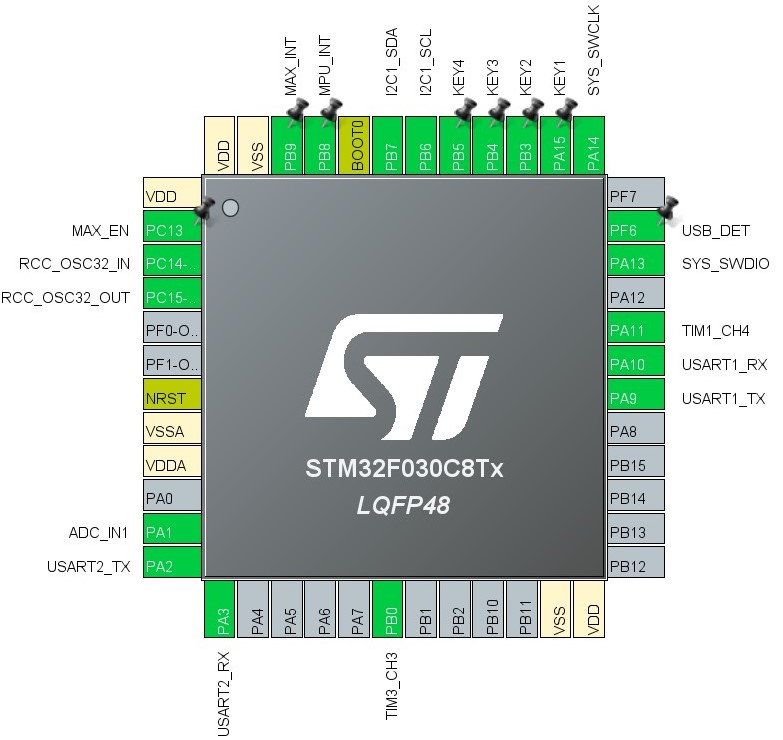
\includegraphics[width=0.9\linewidth]{cube}
		\caption{نحوه‌ی تخصیص پایه‌های مختلف ریزپردازنده در نرم‌افزار \lr{CubeMX}}
		\label{fig:cube-main}
	\end{figure}

\subsection{کلاک}
تنظیمات کلاک به صورت شکل \ref{fig:cube-rcc} است. نوسان‌ساز اصلی روی 8 مگاهرتز داخلی تنظیم شده است و برای ایجاد کلاک بخش ساعت و تاریخ، از یک کریستال خارجی با فرکانس 768.32 کلیوهرتز استفاده شده است. کلاک بخش‌های مختلف نیز در همین تصویر قابل مشاهده است.

	\begin{figure}[h]
		\centering
		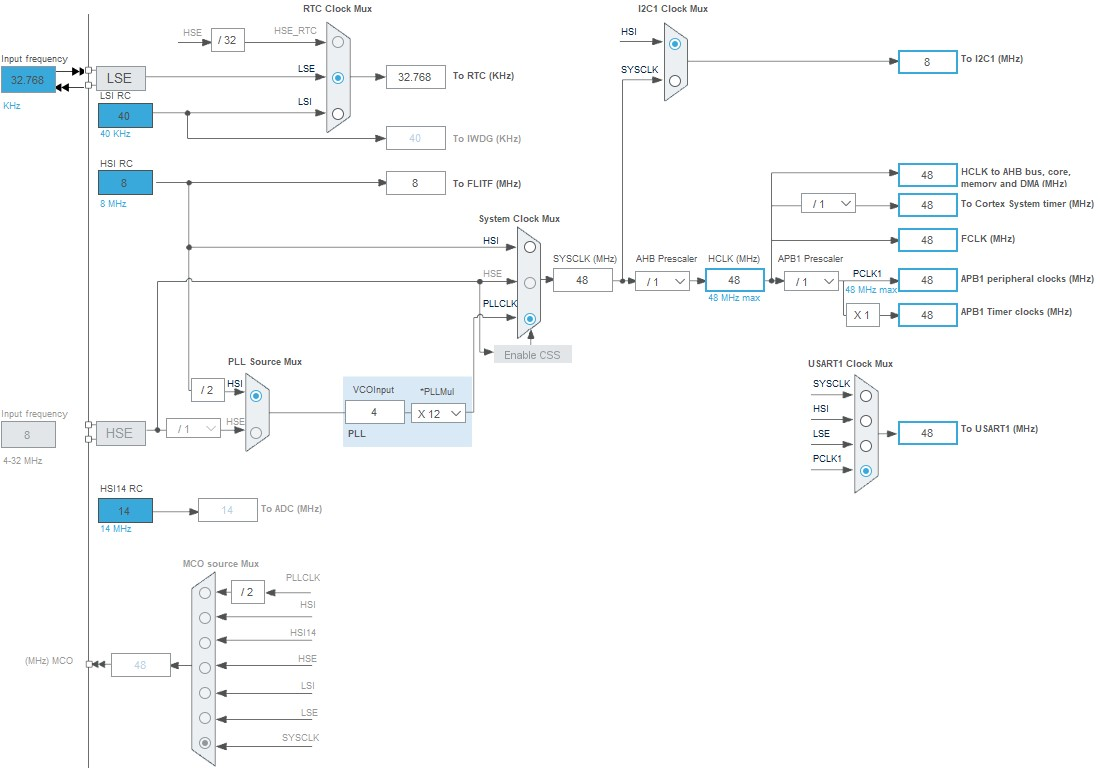
\includegraphics[width=0.9\linewidth]{cube_rcc}
		\caption{تنظیمات کلاک}
		\label{fig:cube-rcc}
	\end{figure}

\subsection{برنامه‌ریزی و اشکال‌زدایی}
برای بحث برنامه‌ریزی\footnote{انتقال برنامه‌ی نوشته شده به ریزپردازنده یا به اصطلاح \lr{Programming}} و اشکال‌زدایی\footnote{\lr{Debugging}} از پروتکل \lr{Serial Wire} استفاده شده است که در شکل \ref{fig:cube-sys} تنظیم آن دیده می‌شود.

	\begin{figure}[h]
		\centering
		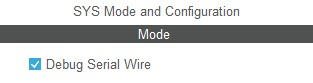
\includegraphics[width=0.4\linewidth]{cube_sys}
		\caption{تنظیمات \lr{Debugging}}
		\label{fig:cube-sys}
	\end{figure}

\subsection{\lr{GPIO}}\label{sec:gpio}
\lr{GPIO}ها پایه‌هایی هستند که به عنوان ورودی/خروجی دیجیتال مورد استفاده قرار می‌گیرند. در این پروژه از \lr{GPIO}های متعددی استفاده شده است که در شکل \ref{fig:cube-gpio} فهرست آن‌ها قابل مشاهده است. در ادامه هر مورد توضیح داده می‌‌شود.

	\begin{figure}[h]
		\centering
		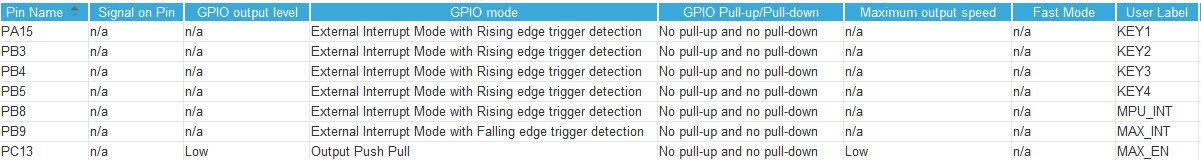
\includegraphics[width=\linewidth]{cube_gpio}
		\caption{تنظیمات \lr{GPIO}}
		\label{fig:cube-gpio}
	\end{figure}

\subsubsection{وقفه‌های خارجی}
وقفه‌های خارجی\footnote{\lr{External intrrupts}}
پایه‌هایی هستند که در صورت وقوع رویداد خاصی، کار عادی پردازنده را متوقف می‌کنند و یک تابع به خصوص را به اجرا در می‌آورند. بعد از اجرای روتین وقفه، پردازنده به کار قبلی خود ادامه می‌دهد.

رویدادهای مورد استفاده در این پروژه دو مورد است: 1- لبه‌ی پایین رونده\footnote{\lr{Falling Edge}}
2- لبه‌ی بالا رونده\footnote{\lr{Rising Edge}}
همانطور که در شکل \ref{fig:cube-gpio} مشهود است، پایه‌های 3، 4، 5 و 8 از پورت \lr{B} و پایه‌ی 15 از پورت \lr{A} برای لبه‌ی بالارونده تنظیم شده‌اند. پایه‌ی 9 از پورت \lr{B} نیز به لبه‌ی پایین رونده حساس است.

اینکه کدام پایه توسط کدام بخش تحریک می‌شود در ستون \lr{User label} شکل \ref{fig:cube-gpio} دیده می‌شود. برچسب‌های \lr{KEY} مربوطه به کلیدهای لمسی روی بدنه هستند. در صورت لمس شدن هر کلید، تابع مخصوص آن اجرا می‌شود. برچسب \lr{MPU} مربوط به حسگر حرکتی است. این پایه وقتی فعال می‌شود که داده‌های جدید حسگر آماده شده باشد. برچسب \lr{MAX} نیز به همین شکل عمل می‌کند. هرگاه داده‌ی حسگر \lr{PPG} آماده‌ی قرائت باشد، این وقفه فعال می‌شود.

\subsubsection{خروجی دیجیتال}
پایه‌ی 13 از پورت \lr{C} به صورت خروجی دیجیتال تعریف شده است. این خروجی به پایه‌ی فعالساز سوییچ ماسفتی متصل است که حسگر \lr{PPG} را روشن می‌کند (شکل \ref{fig:sch-ppg}). برای روشن یا خاموش کردن این حسگر، کافی است این پایه را صفر یا یک کرد.

\subsection{\lr{RTC}}
واحد
\lr{RTC}\footnote{\lr{Real-time Clock}}
برای نگهداری و کار با ساعت و تاریخ است. تنظیمات این بخش در شکل \ref{fig:cube-rtc} دیده می‌شود. در این بخش می‌توان یک آلارم هم فعال کرد که در ساعت و روز مشخصی یک وقفه را فعال کند. در اینجا آلارم هم فعال شده است.

	\begin{figure}[h]
		\centering
		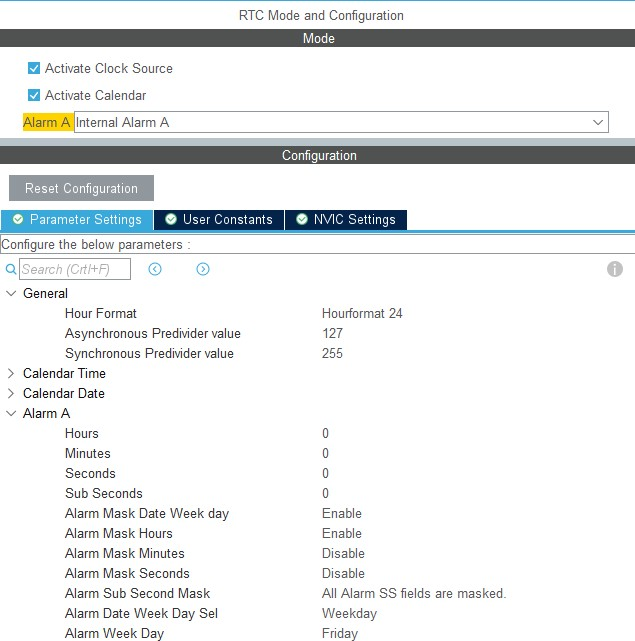
\includegraphics[width=0.45\linewidth]{cube_rtc}
		\caption{تنظیمات \lr{RTC}}
		\label{fig:cube-rtc}
	\end{figure}

\subsection{تایمرها}
این ریزپردازنده هفت تایمر دارد که در این پروژه هر هفت تایمر استفاده شده‌اند. در ادامه کاربرد و تنظیمات هر تایمر شرح داده می‌شود.

\subsubsection{\lr{TIM1}}
تایمر شماره‌ی یک مطابق با تنظیمات شکل \ref{fig:cube-tim1} راه‌اندازی شده است تا بتواند \lr{PWM} موردنیاز برای کنترل دور موتور ایجاد لرزش را تولید کند. البته مقدار رجیستر
\lr{ARR}\footnote{\lr{Auto-Reload Register} رجیستری است که برای تنظیم فرکانس اصلی تایمر استفاده می‌شود}
در برنامه به صورت پویا تغییر می‌کند.

\subsubsection{\lr{TIM3}}
تایمر شماره‌ی یک مطابق با تنظیمات شکل \ref{fig:cube-tim3} راه‌اندازی شده است تا بتواند \lr{PWM} موردنیاز برای تنظیم فرکانس صدای بازر را تولید کند. البته مقدار رجیستر
\lr{ARR}
در برنامه به صورت پویا تغییر می‌کند.

	\begin{figure}[h]
		\centering
		\begin{subfigure}{0.4\textwidth}
			\centering
			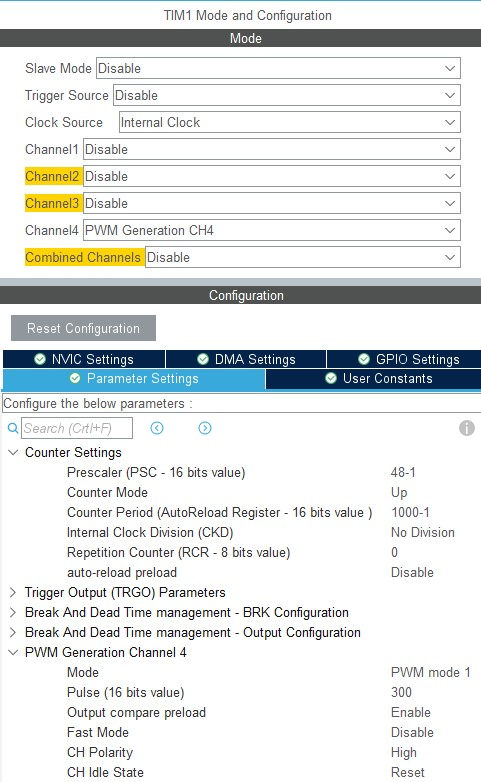
\includegraphics[width=\linewidth]{cube_tim1}
			\caption{تنظیمات تایمر یک}
			\label{fig:cube-tim1}
		\end{subfigure}
		\begin{subfigure}{0.44\textwidth}
			\centering
			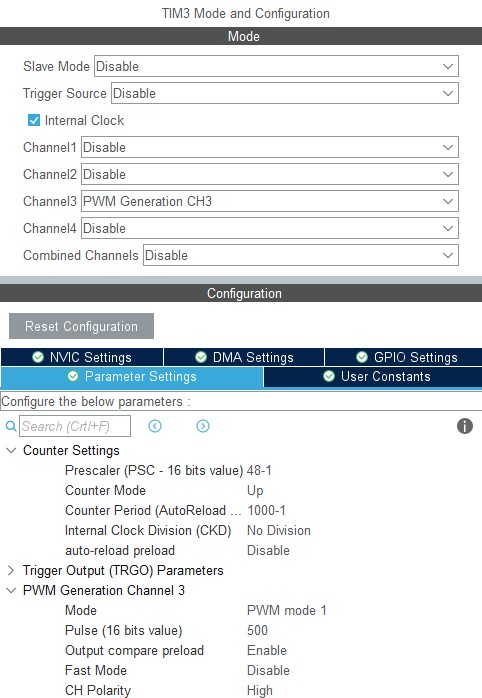
\includegraphics[width=\linewidth]{cube_tim3}
			\caption{تنظیمات تایمر سه}
			\label{fig:cube-tim3}
		\end{subfigure}
		\caption{تنظیمات دو تایمر}
		%\label{fig:body-pcb}
	\end{figure}

\subsubsection{\lr{TIM6}}
تایمر شماره‌ی شش مطابق شکل \ref{fig:cube-tim6} تنظیم شده است تا هر یک میلی ثانیه یک وقفه را فعال کند. این وقفه توابع مربوط به فیلتر کالمن را اجرا می‌کند. در واقع می‌توان گفت دوره تناوب نمونه‌گیری و پردازش سیستم کالمن یک میلی ثانیه است.

	\begin{figure}[h]
		\centering
		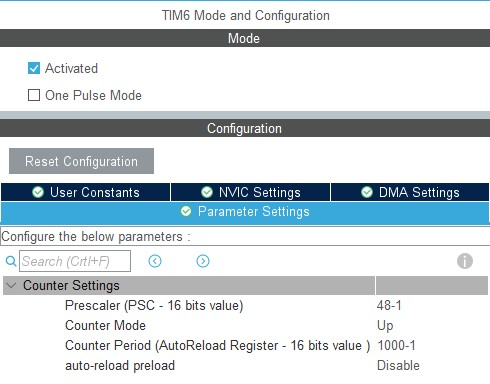
\includegraphics[width=0.43\linewidth]{cube_tim6}
		\caption{تنظیمات تایمر شش}
		\label{fig:cube-tim6}
	\end{figure}

\subsubsection{\lr{TIM14}}
تایمر شماره‌ی چهارده مطابق شکل \ref{fig:cube-tim14} تنظیم شده است تا هر 250 میلی ثانیه یک وقفه را فعال کند. این وقفه مربوط به توابع سیستمی است. در این توابع مواردی از قبیل تازه‌سازی صفحه نمایش و تنظیم برخی متغیرها انجام می‌شود.


	\begin{figure}[h]
		\centering
		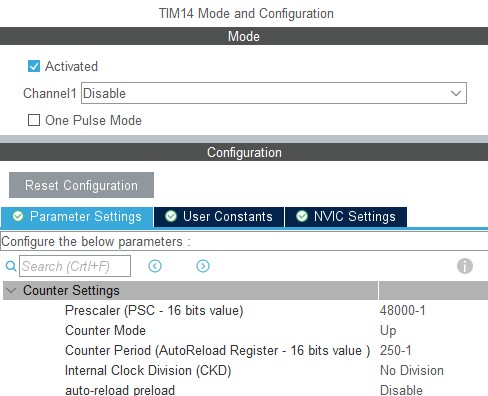
\includegraphics[width=0.35\linewidth]{cube_tim14}
		\caption{تنظیمات تایمر چهارده}
		\label{fig:cube-tim14}
	\end{figure}

\subsubsection{\lr{TIM15}}
تایمر شماره‌ی پانزده مطابق شکل \ref{fig:cube-tim15} تنظیم شده است تا هر 10 میلی ثانیه به واحد \lr{ADC} فرمانِ تبدیل دهد. به این معنی که واحد آنالوگ به دیجیتال فقط در صورتی یک نمونه‌برداری را شروع می‌کند که تایمر شماره 15 به آن فرمان دهد. اینگونه یک نمونه‌برداری دقیق زمانی ایجاد می‌شود.

	\begin{figure}[h]
		\centering
		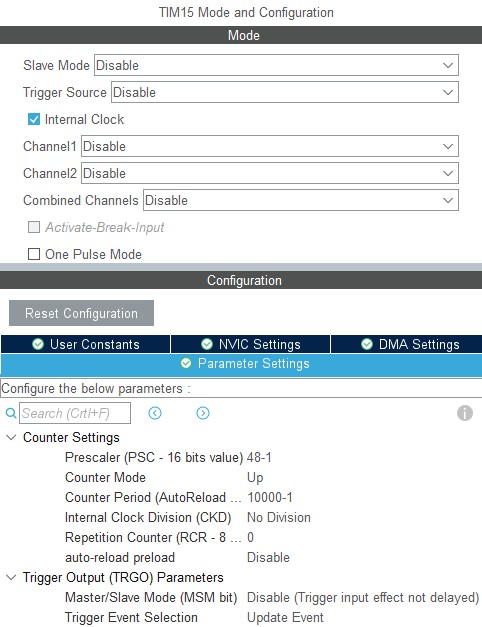
\includegraphics[width=0.4\linewidth]{cube_tim15}
		\caption{تنظیمات تایمر پانزده}
		\label{fig:cube-tim15}
	\end{figure}

\subsubsection{\lr{TIM16}}
تایمر شماره‌ی شانزده مطابق شکل \ref{fig:cube-tim16} تنظیم شده است تا هر 4 ثانیه یک وقفه را فعال کند. این وقفه برای خاموش کردن صفحه نمایش است. هرگاه کاربر به مدت 4 ثانیه با ساعت تعامل نداشته باشد این وقفه صفحه را خاموش می‌کند.

	\begin{figure}[h]
		\centering
		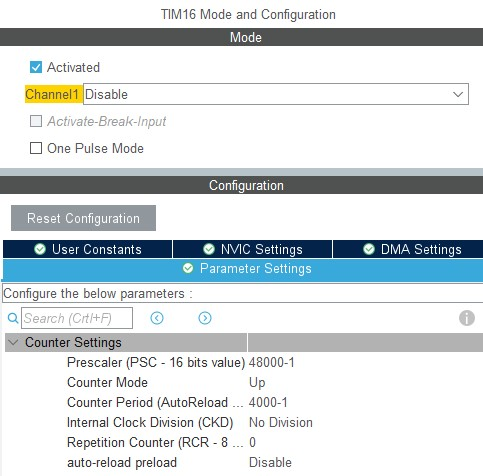
\includegraphics[width=0.4\linewidth]{cube_tim16}
		\caption{تنظیمات تایمر شانزده}
		\label{fig:cube-tim16}
	\end{figure}

\subsubsection{\lr{TIM17}}
تایمر شماره‌ی هفده مطابق شکل \ref{fig:cube-tim17} تنظیم شده است. این تایمر وقفه ندارد و به صورت یک زمان‌سنج به کار می‌رود. از این تایمر برای ساخت تابع تأخیر استفاده شده است. حداکثر تأخیر قابل تولید توسط این تایمر، دو به توان 16 یعنی 65536 میلی ‌ثانیه است. 

	\begin{figure}[h]
		\centering
		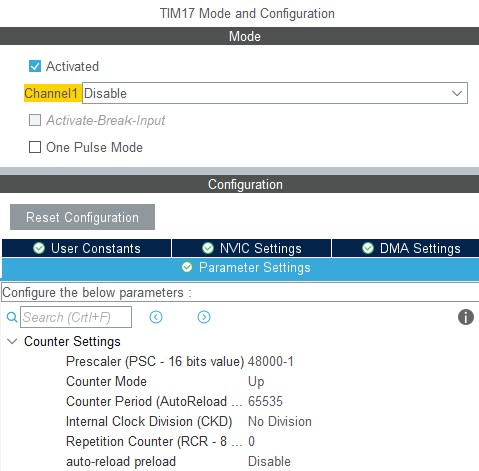
\includegraphics[width=0.4\linewidth]{cube_tim17}
		\caption{تنظیمات تایمر هفده}
		\label{fig:cube-tim17}
	\end{figure}

\subsection{\lr{ADC}}
مبدل آنالوگ به دیجیتال در این پردازنده 12 بیتی است. یعنی ولتاژ ورودی را از بازه‌ی 0 تا 3.3 ولت به بازه‌ی 0 تا 4095 نگاشت می‌کند. اینگونه می‌توان با یک ضرب و تقسیم ساده مقدار ولتاژ ورودی را خواند. شکل \ref{fig:cube-adc} تنظیمات این واحد را نشان می‌دهد. همانطور که گفته شد، این واحد به کمک تایمر 15 فعال می‌شود و با هر فرمان آن یک نمونه برمی‌دارد. برای ذخیره‌ی این نمونه‌ها، \lr{ADC} را با
\lr{DMA}\footnote{\lr{Direct Memory Access}}
کوپل می‌کنیم. اینگونه هربار که \lr{ADC} یک نمونه را تبدیل کرد، به طور مستقیم و بدون دخالت پردازنده آن را در یک آرایه ذخیره می‌کند. بعد از اینکه آرایه پر شد نیز با فعال کردن یک وقفه به ما خبر می‌دهد تا عملیات پردازشی روی آن انجام گیرد.

این ساختار که \lr{ADC} با تایمر فعال شود و با \lr{DMA} کار کند، حرفه‌ای ترین ساختار راه‌اندازی این واحد است. تنظیمات \lr{DMA} در شکل \ref{fig:cube-adc-dma} دیده می‌شود.

	\begin{figure}[h]
		\centering
		\begin{subfigure}{0.5\textwidth}
			\centering
			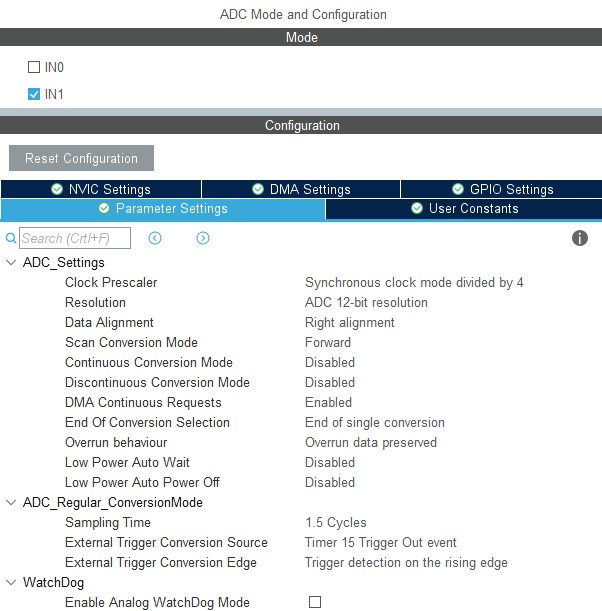
\includegraphics[width=\linewidth]{cube_adc}
			\caption{تنظیمات \lr{ADC}}
			\label{fig:cube-adc}
		\end{subfigure} \\
		\begin{subfigure}{0.54\textwidth}
			\centering
			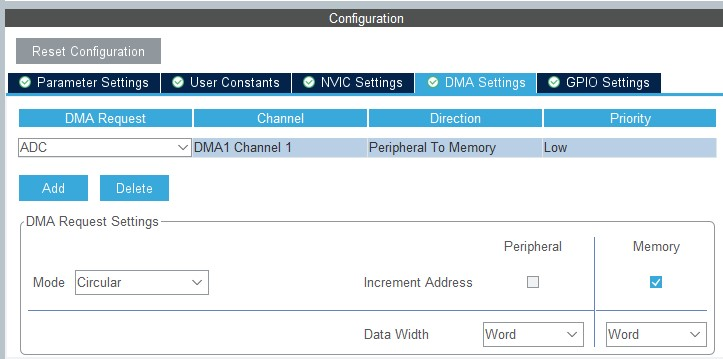
\includegraphics[width=\linewidth]{cube_adc_dma}
			\caption{تنظیمات \lr{DMA}}
			\label{fig:cube-adc-dma}
		\end{subfigure}
		\caption{تنظیمات مبدل آنالوگ به دیجیتال}
	\end{figure}

\subsection{\lr{I2C}}
واحد \lr{I2C} مطابق شکل \ref{fig:cube-i2c} تنظیم شده است. این واحد یک واحد ارتباطی تحت پروتکل \lr{I2C} است.

	\begin{figure}[h]
		\centering
		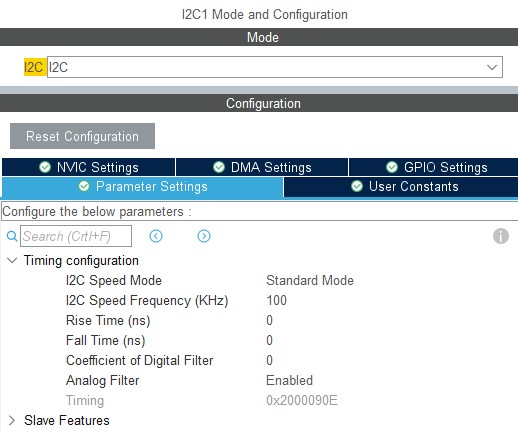
\includegraphics[width=0.5\linewidth]{cube_i2c}
		\caption{تنظیمات \lr{I2C}}
		\label{fig:cube-i2c}
	\end{figure}

\subsection{\lr{USART}}
واحد \lr{USART1} و \lr{USART2} مطابق شکل \ref{fig:cube-usart} تنظیم شده و تنظیمات مشابهی دارند. با این تفاوت که \lr{USART2} به یک واحد \lr{DMA} نیز وصل است تا داده‌ی دریافتی بلوتوث را مستقیماً در حافظه ذخیره کند و در صورت تکمیل شدن پیام، وقفه‌ی مربوطه را فعال کند تا داده‌ی دریافتی پردازش شود.

	\begin{figure}[h]
		\centering
		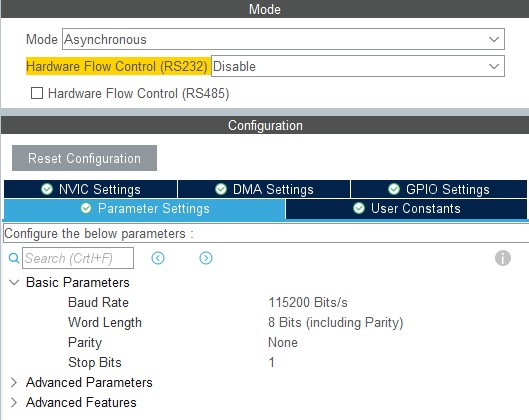
\includegraphics[width=0.5\linewidth]{cube_usart}
		\caption{تنظیمات \lr{USART}}
		\label{fig:cube-usart}
	\end{figure}



\section{معماری}
برنامه‌ی نوشته شده در این پروژه مشابه برنامه‌های عادی ریزپردازنده‌ها نیست. در اکثر قریب به اتفاق پروژه‌ها، معماری به این صورت است که ابتدا چند تابع اجرا می‌شوند تا تنظیمات کلی را انجام دهند، سپس یک حلقه‌ی \lr{while(1)} وجود دارد تا روتین اصلی برنامه به صورت مداوم در آن اجرا شود. در این معماری وظیفه‌های\footnote{\lr{Tasks}}
مختلف به طور غیر همزمان اجرا شده و مشکلات زمان‌بندی دارند.

اما معماری این پروژه یک معماری رویداد محور\footnote{\lr{Event-based architecture}}
است. در این معماری حلقه‌ی \lr{while(1)} خالی است و تمام وظیفه‌ها در توابع وقفه رسیدگی می‌شوند.

در کنار این معماری رویداد محور، یک ماشین حالت محدود یا به اختصار
\lr{FSM}\footnote{\lr{Finite State Machine}}
نیز وجود دارد تا حالت‌های کاری مختلف را اجرا کند.

در ادامه بخش‌های مختلف این معماری شرح داده می‌شود.
\subsection{ماشین حالت} \label{sec:fsm}
ماشین حالت مفهومی است برای توصیف و تشریح عملکرد یک سیستم که حالت‌های کاری مختلفی دارد. این مفهوم نشان می‌دهد که چگونه هر حالت به حاتی دیگر تبدیل می‌شود و در هر حالت خروجی سیستم چیست.

	\begin{figure}[h]
		\centering
		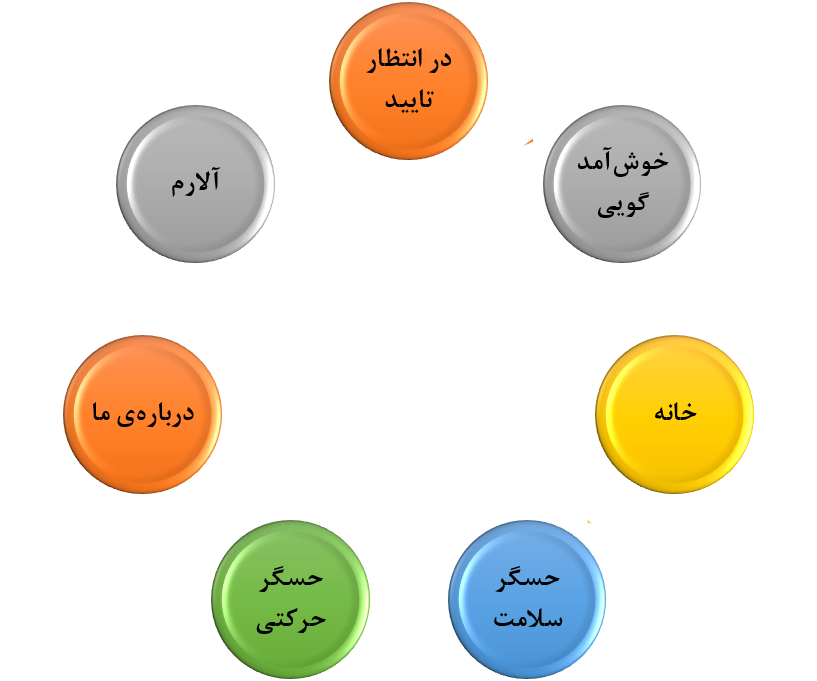
\includegraphics[width=0.5\linewidth]{states}
		\caption{حالت‌های ماشین حالت}
		\label{fig:states}
	\end{figure}

در این پروژه ماشین حالت را تعمیم داده‌ام. به این صورت که انتقال بین حالت‌ها همچنان به کمک یک سیگنال کلاک صورت می‌گیرد، اما دیگر هر حالت خروجی ثابتی ندارد، بلکه مجموعه‌ای ای توابع در هر حالت دائماً اجرا می‌شوند. شکل \ref{fig:states} حالت‌ها و نام آن‌ها را نشان می‌دهد.

\subsubsection{حالت در انتظار تایید}
\begin{itemize}
	\item روتین اصلی:
		\begin{enumerate}
			\item نمایش صفحه‌ی درخواست تایید مطابق شکل \ref{fig:state-ack}
			\item متوقف کردن تایمر خاموش کردن صفحه نمایش
		\end{enumerate}
	\item کلید بالا فشرده شود:
		\begin{enumerate}
			\item یک کردن متغیر \lr{ack} در ساختار سیستم
			\item فراخوانی تابع سیستمی ارسال تاییدیه
		\end{enumerate}
	\item کلید پایین فشرده شود:
		\begin{enumerate}
			\item صفر کردن متغیر \lr{ack} در ساختار سیستم
			\item فراخوانی تابع سیستمی ارسال عدم تایید
			\item تنظیم حالت روی خانه
			\item فعال کردن صفحه نمایش
		\end{enumerate}
\end{itemize}
	\begin{figure}[h]
		\centering
		
\includegraphics[width=0.5\linewidth]{state_ack}
		\caption{صفحه‌ی در انتظار تایید}
		\label{fig:state-ack}
	\end{figure}

\subsubsection{حالت خوش‌آمد گویی}
\begin{itemize}
	\item روتین اصلی:
	\begin{enumerate}
		\item نمایش صفحه‌ی خوش‌آمد گویی به مدت 4 ثانیه \ref{fig:state-hello}
		\item تنظیم حالت به عنوان خانه
		\item فعال کردن تایمر خاموش کردن صفحه
	\end{enumerate}
\end{itemize}
	\begin{figure}[h]
		\centering
		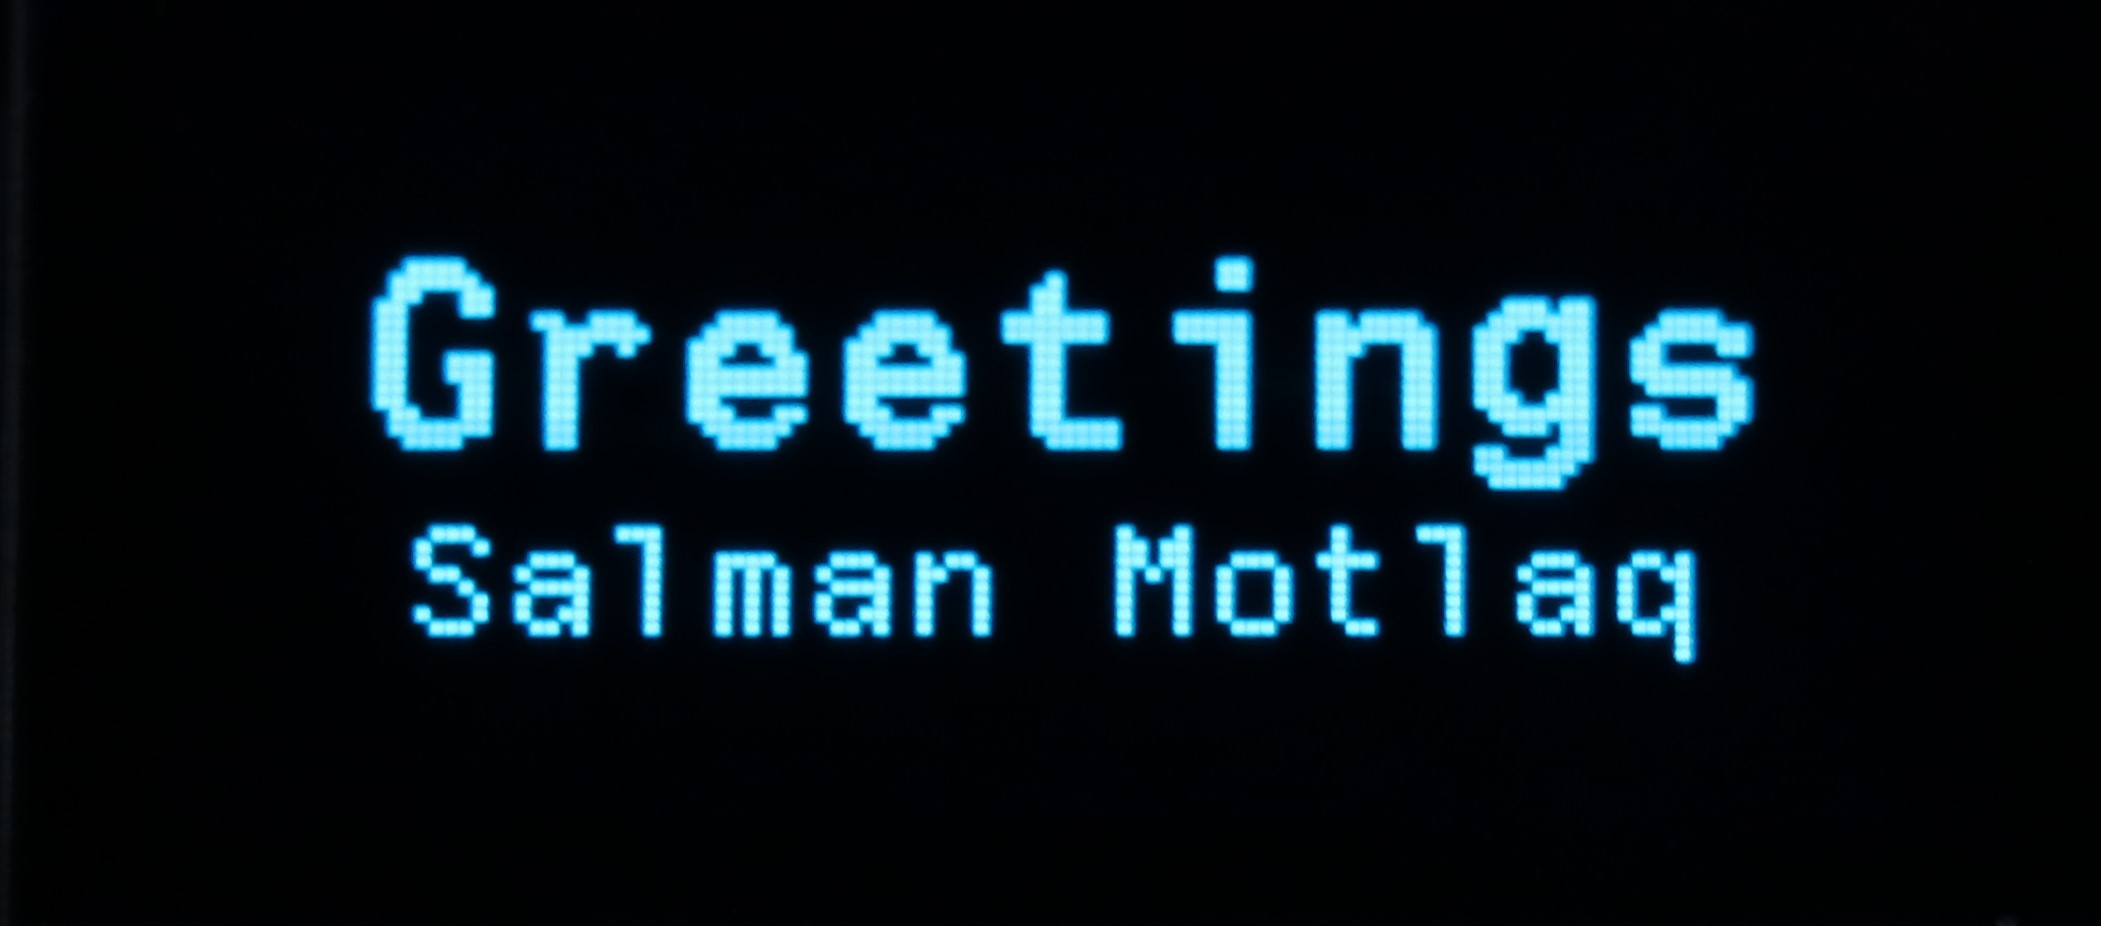
\includegraphics[width=0.5\linewidth]{state_hello}
		\caption{صفحه‌ی خوش‌آمد گویی}
		\label{fig:state-hello}
	\end{figure}

\subsubsection{حالت خانه}
\begin{itemize}
	\item روتین اصلی:
	\begin{enumerate}
		\item قرائت ساعت و تاریخ
		\item قرائت میزان شارژ باتری
		\item قرائت وضعیت اتصال به گوشی
		\item نمایش صفحه‌ی اصلی مطابق شکل \ref{fig:state-home}
	\end{enumerate}
	\item کلید بالا فشرده شود:
	\begin{enumerate}
		\item تنظیم حالت روی درباره‌ی ما
	\end{enumerate}
	\item کلید پایین فشرده شود:
	\begin{enumerate}
		\item متوقف کردن تایمر فیلتر کالمن
		\item متوقف کردن تایمر \lr{ADC}
		\item روشن کردن حسگر \lr{PPG} و تنظیم آن
		\item تنظیم حالت روی حسگر سلامت
	\end{enumerate}
\end{itemize}
	\begin{figure}[h]
		\centering
		\begin{subfigure}{0.4\textwidth}
			\centering
			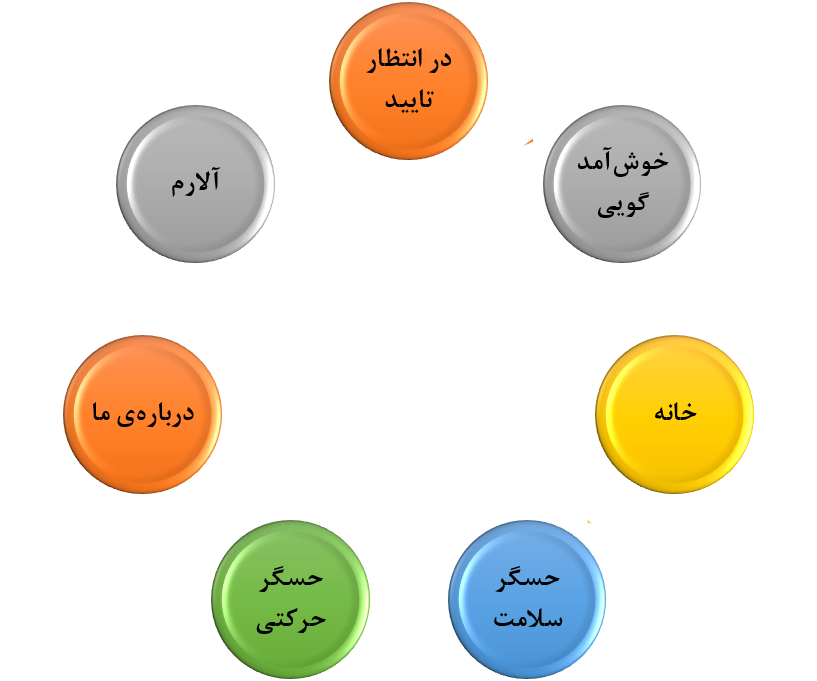
\includegraphics[width=\linewidth]{state_home}
			\caption{در حالتی که اتصال با گوشی برقرار است}
			%\label{fig:oled_image}
		\end{subfigure}
		\begin{subfigure}{0.4\textwidth}
			\centering
			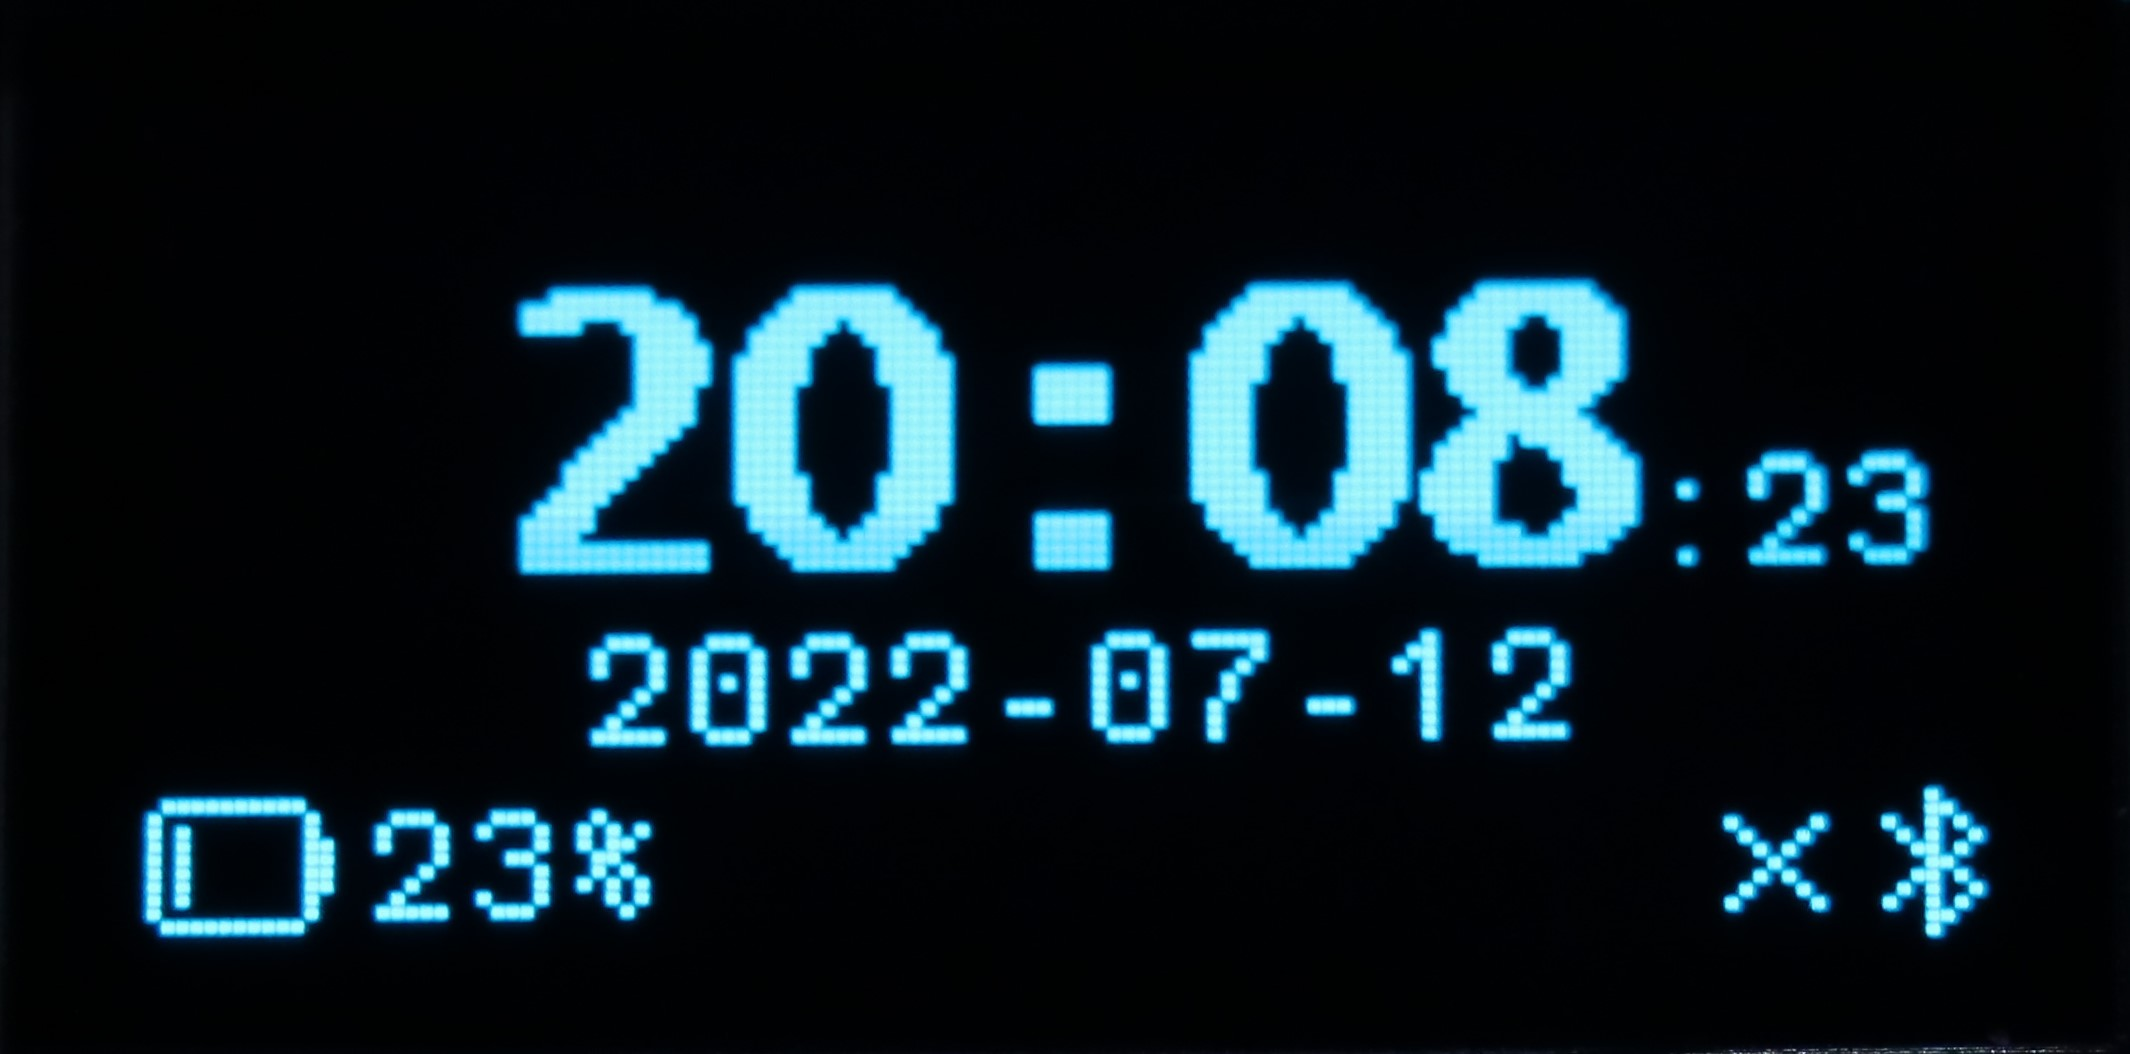
\includegraphics[width=0.95\linewidth]{state_home_nc}
			\caption{در حالتی که اتصال با گوشی برقرار نیست}
			%\label{fig:oled_real}
		\end{subfigure}
		\caption{صفحه‌ی اصلی}
		\label{fig:state-home}
	\end{figure}

\subsubsection{حالت حسگر سلامت}
\begin{itemize}
	\item روتین اصلی:
	\begin{enumerate}
		\item نمایش صفحه‌ی حسگر سلامت مطابق شکل \ref{fig:state-bloody}
		\item متوقف کردن تایمر خاموش کردن صفحه نمایش
	\end{enumerate}
	\item کلید بالا فشرده شود:
	\begin{enumerate}
		\item خاموش کردن حسگر سلامت
		\item روشن کردن تایمر فیلتر کالمن
		\item روشن کردن تایمر \lr{ADC}
		\item روشن کردن تایمر خاموش شدن صفحه نمایش
		\item تنظیم حالت روی خانه
	\end{enumerate}
	\item کلید پایین فشرده شود:
	\begin{enumerate}
		\item خاموش کردن حسگر سلامت
		\item روشن کردن تایمر فیلتر کالمن
		\item روشن کردن تایمر \lr{ADC}
		\item تنظیم حالت روی حسگر حرکتی
	\end{enumerate}
\end{itemize}
	\begin{figure}[h]
		\centering
		\begin{subfigure}{0.4\textwidth}
			\centering
			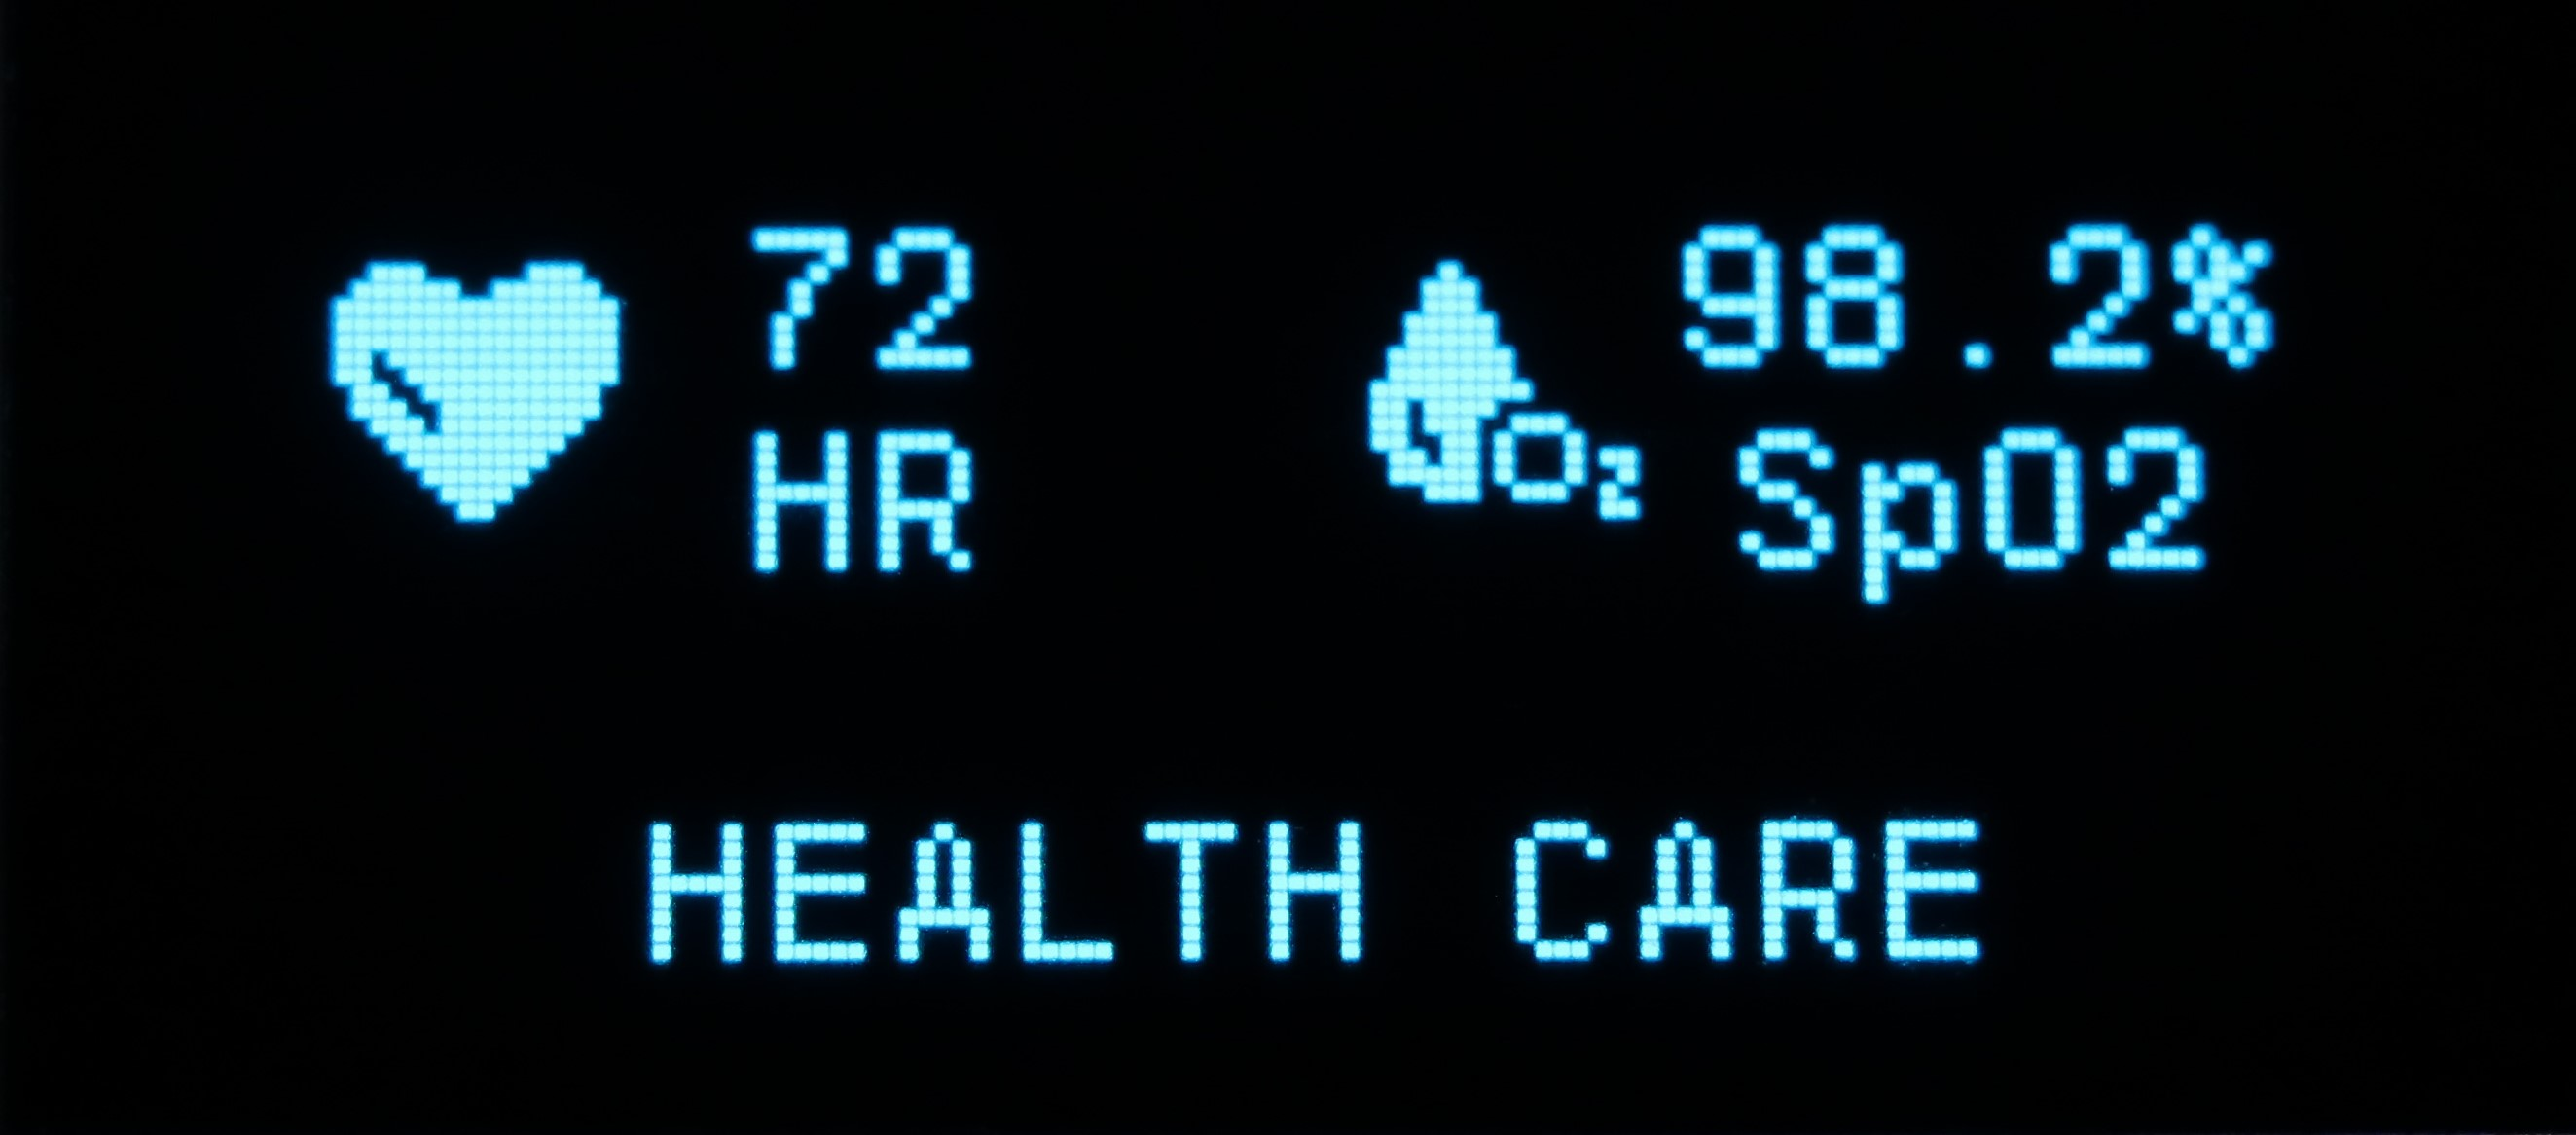
\includegraphics[width=0.98\linewidth]{state_bloody}
			\caption{در حالتی که اتصال با گوشی برقرار است}
			%\label{fig:oled_image}
		\end{subfigure}
		\begin{subfigure}{0.4\textwidth}
			\centering
			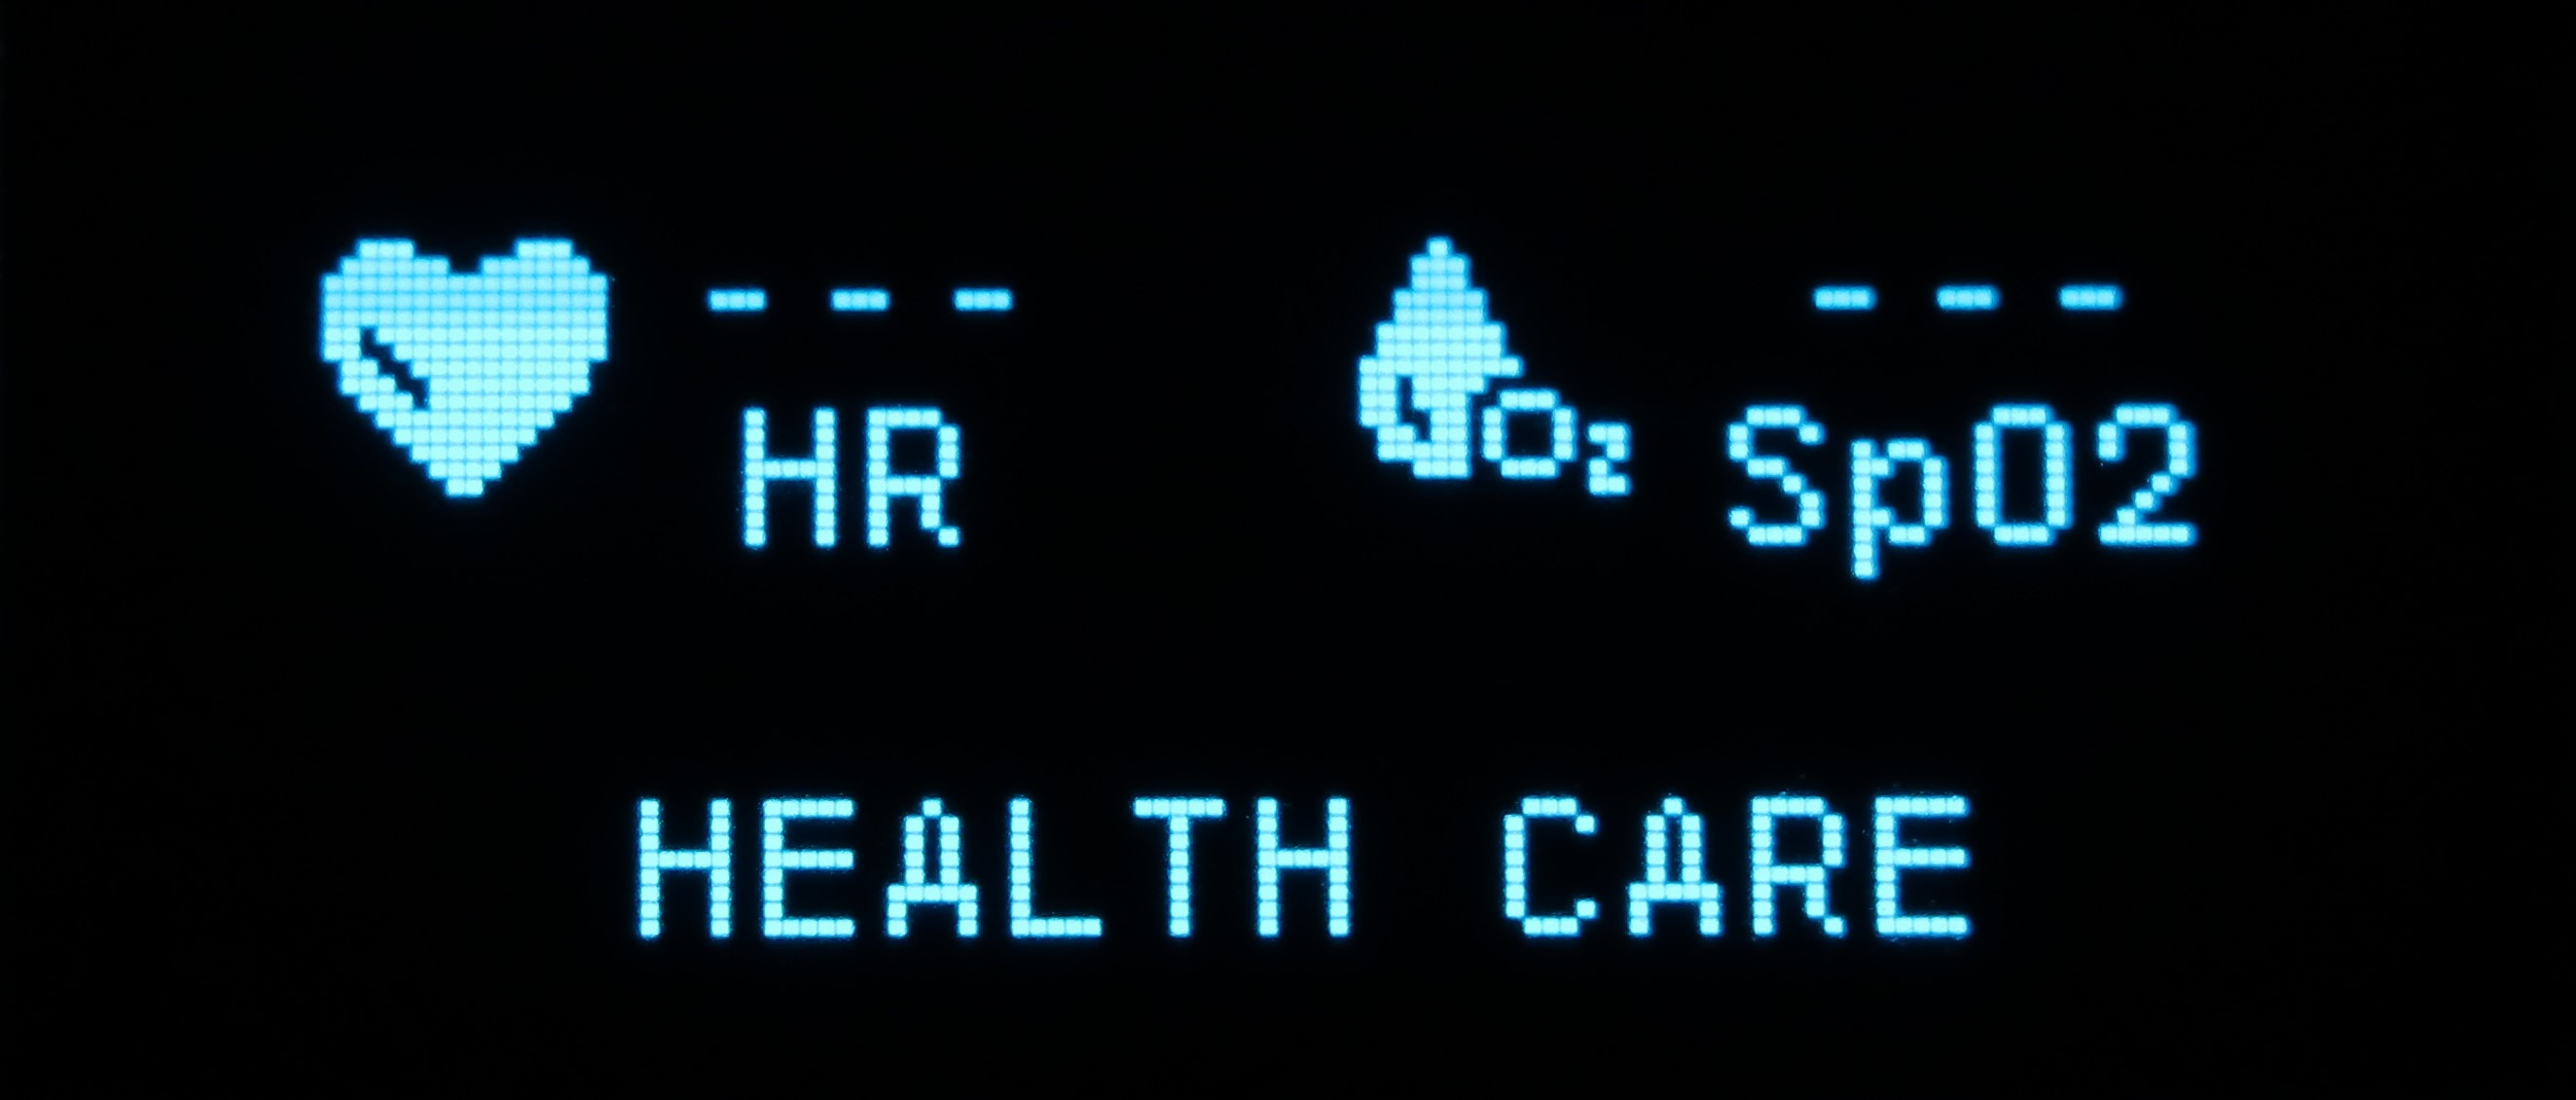
\includegraphics[width=\linewidth]{state_bloody_nc}
			\caption{در حالتی که اتصال با گوشی برقرار نیست}
			%\label{fig:oled_real}
		\end{subfigure}
		\caption{صفحه‌ی حسگر سامت}
		\label{fig:state-bloody}
	\end{figure}
\subsubsection{حالت حسگر حرکتی}
\begin{itemize}
	\item روتین اصلی:
	\begin{enumerate}
		\item نمایش صفحه‌ی حسگر حرکتی مطابق شکل \ref{fig:state-pedomedo}
		\item متوقف کردن تایمر خاموش کردن صفحه نمایش
	\end{enumerate}
	\item کلید بالا فشرده شود:
	\begin{enumerate}
		\item متوقف کردن تایمر فیلتر کالمن
		\item متوقف کردن تایمر \lr{ADC}
		\item روشن کردن حسگر \lr{PPG} و تنظیم آن
		\item تنظیم حالت روی حسگر سلامت
	\end{enumerate}
	\item کلید پایین فشرده شود:
	\begin{enumerate}
		\item تنظیم حالت روی درباره‌ی ما
	\end{enumerate}
\end{itemize}
	\begin{figure}[h]
		\centering
		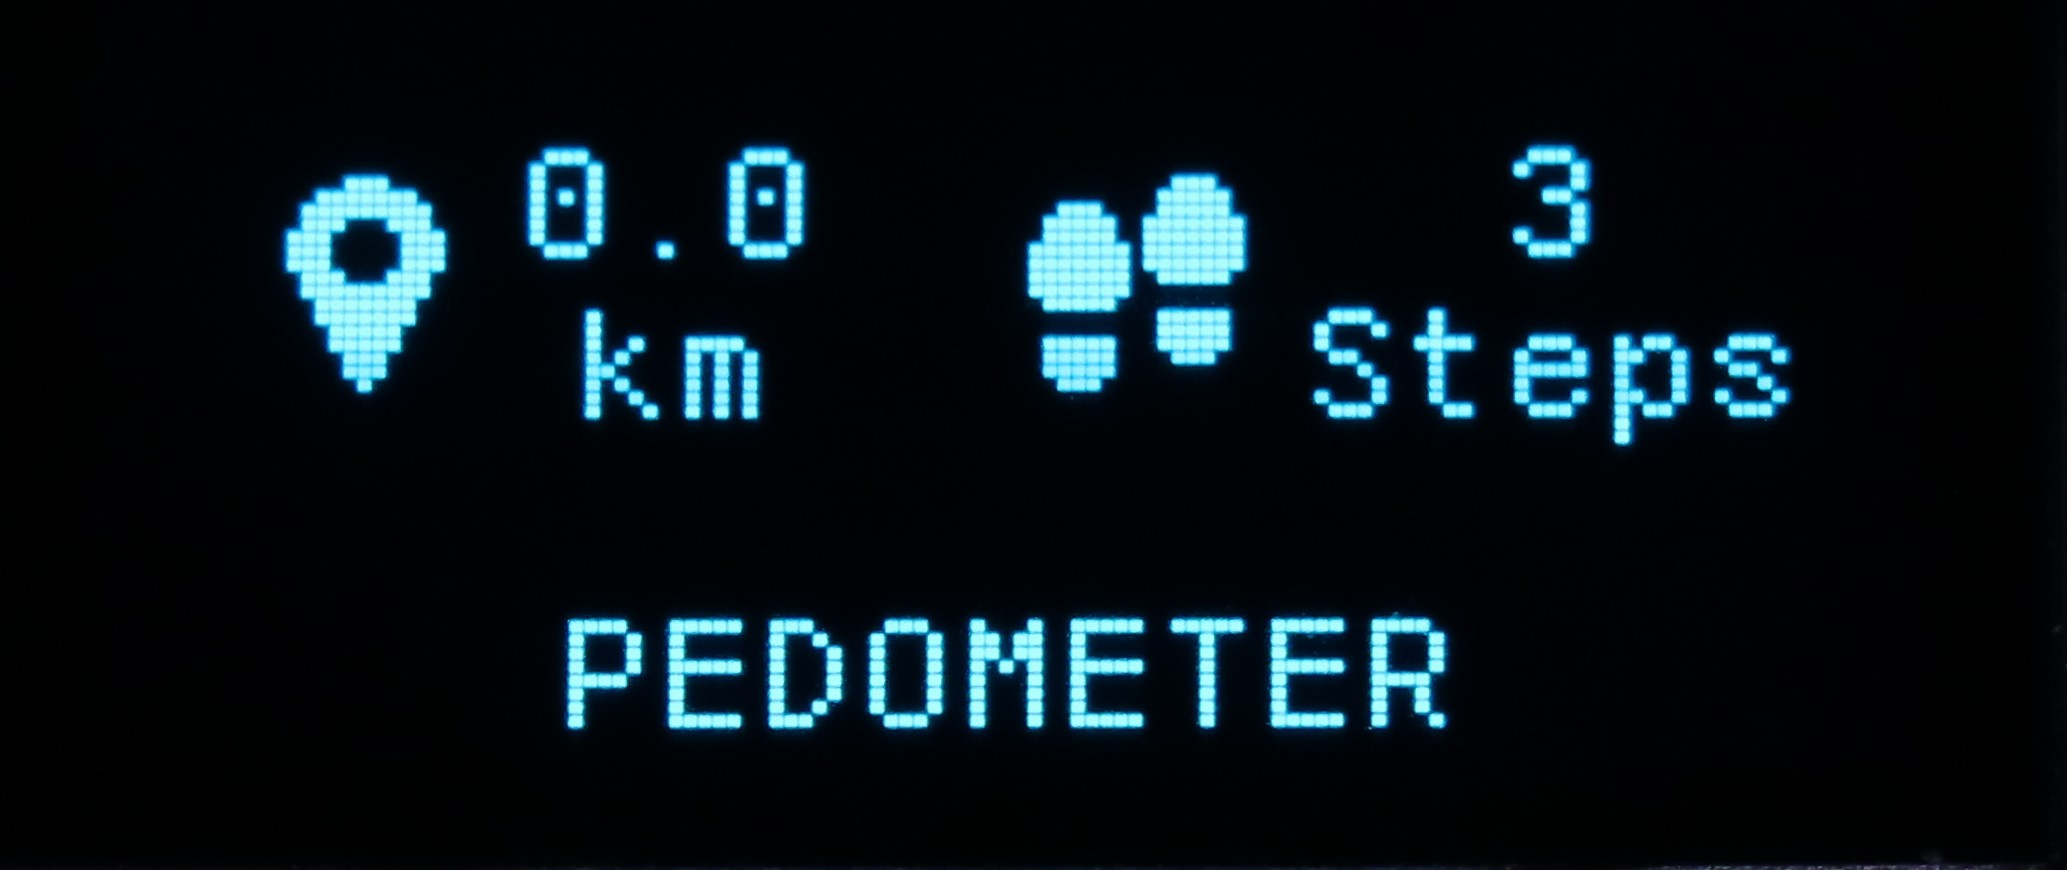
\includegraphics[width=0.5\linewidth]{state_pedomedo}
		\caption{صفحه‌ی حسگر حرکتی}
		\label{fig:state-pedomedo}
	\end{figure}

\subsubsection{حالت درباره‌ی ما}
\begin{itemize}
	\item روتین اصلی:
	\begin{enumerate}
		\item نمایش صفحه‌ی درباره‌ی ما مطابق شکل \ref{fig:state-about}
		\item متوقف کردن تایمر خاموش کردن صفحه نمایش
	\end{enumerate}
	\item کلید بالا فشرده شود:
	\begin{enumerate}
		\item تنظیم حالت روی حسگر حرکتی
	\end{enumerate}
	\item کلید پایین فشرده شود:
	\begin{enumerate}
		\item روشن کردن تایمر خاموش شدن صفحه نمایش
		\item تنظیم حالت روی خانه
	\end{enumerate}
\end{itemize}
	\begin{figure}[h]
		\centering
		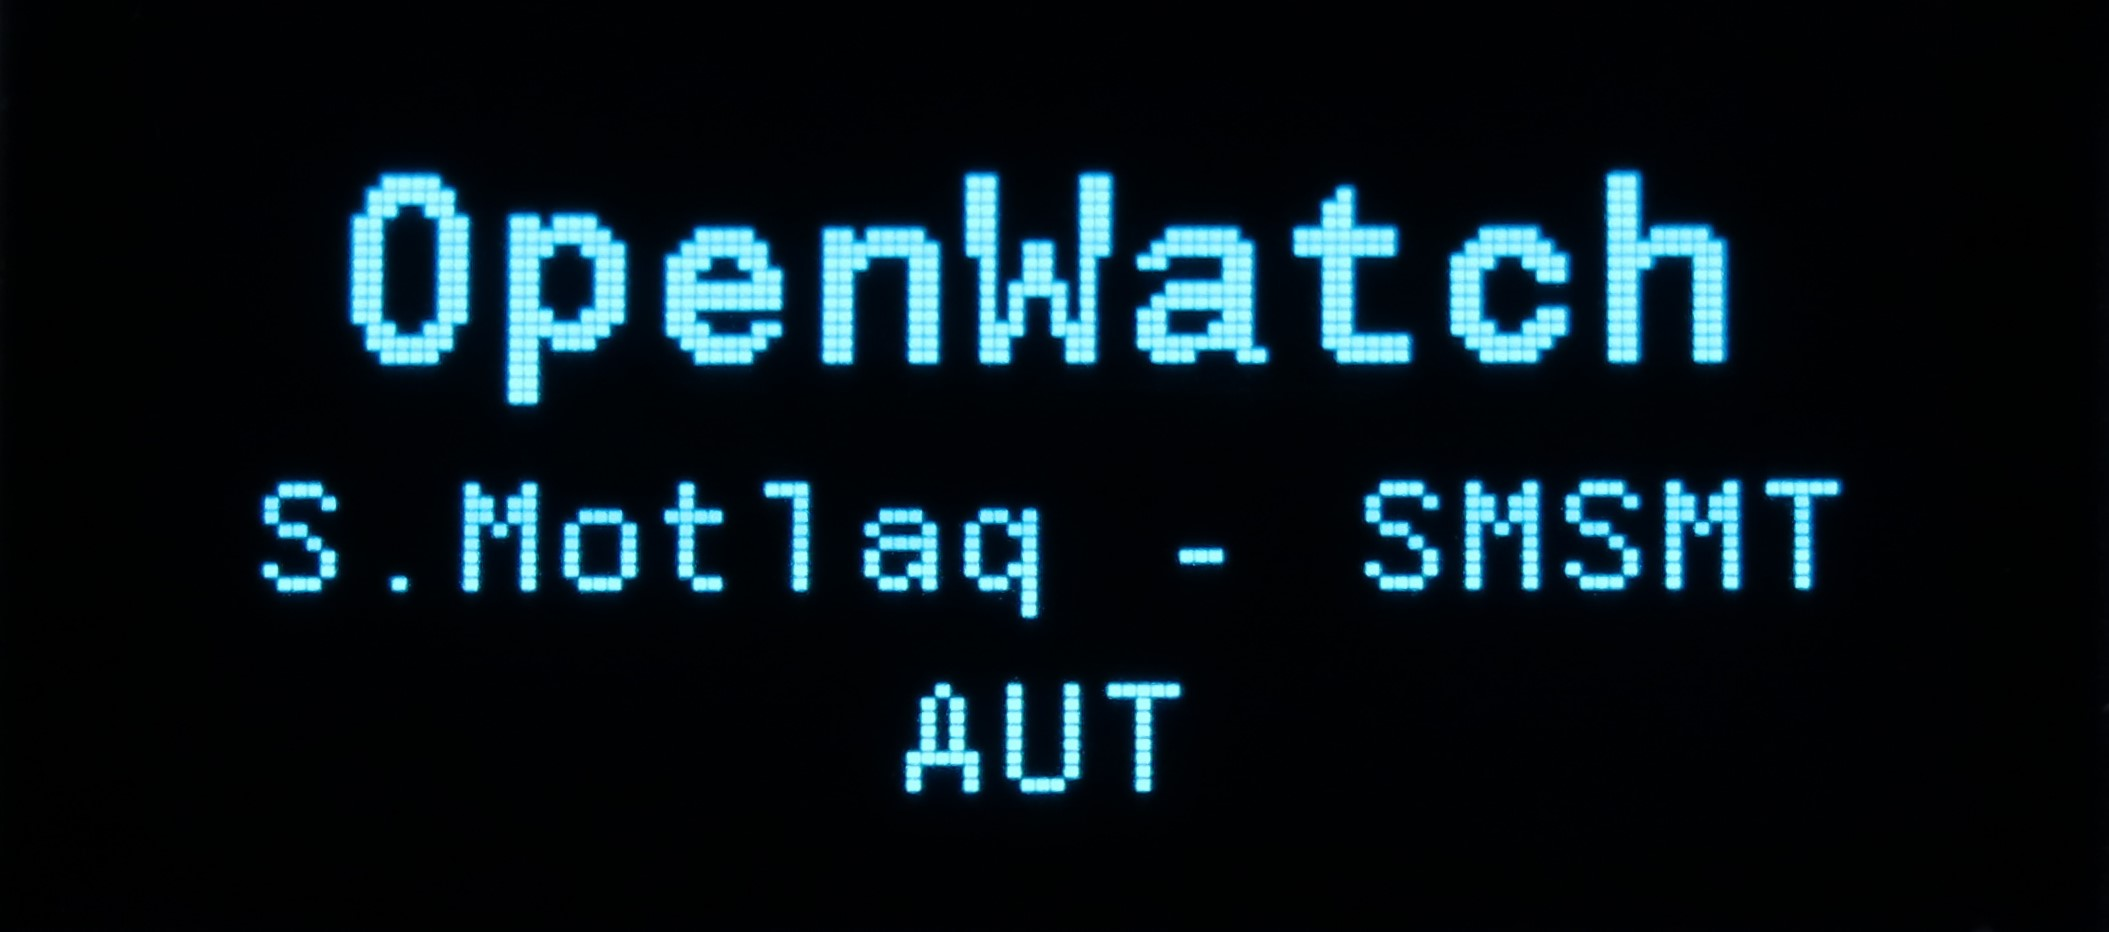
\includegraphics[width=0.5\linewidth]{state_about}
		\caption{صفحه‌ی درباره‌ی ما}
		\label{fig:state-about}
	\end{figure}
\subsubsection{حالت آلارم}
\begin{itemize}
	\item روتین اصلی:
	\begin{enumerate}
		\item نمایش صفحه‌ی آلارم مطابق شکل \ref{fig:state-ringing}
		\item متوقف کردن تایمر خاموش کردن صفحه نمایش
	\end{enumerate}
	\item هر کلیدی که فشرد شود:
	\begin{enumerate}
		\item پایین آوردن پرچم آلارم
		\item روشن کردن تایمر فیلتر کالمن
		\item روشن کردن تایمر خاموش شدن صفحه نمایش
		\item تنظیم حالت روی خانه
	\end{enumerate}
\end{itemize}
	\begin{figure}[h]
		\centering
		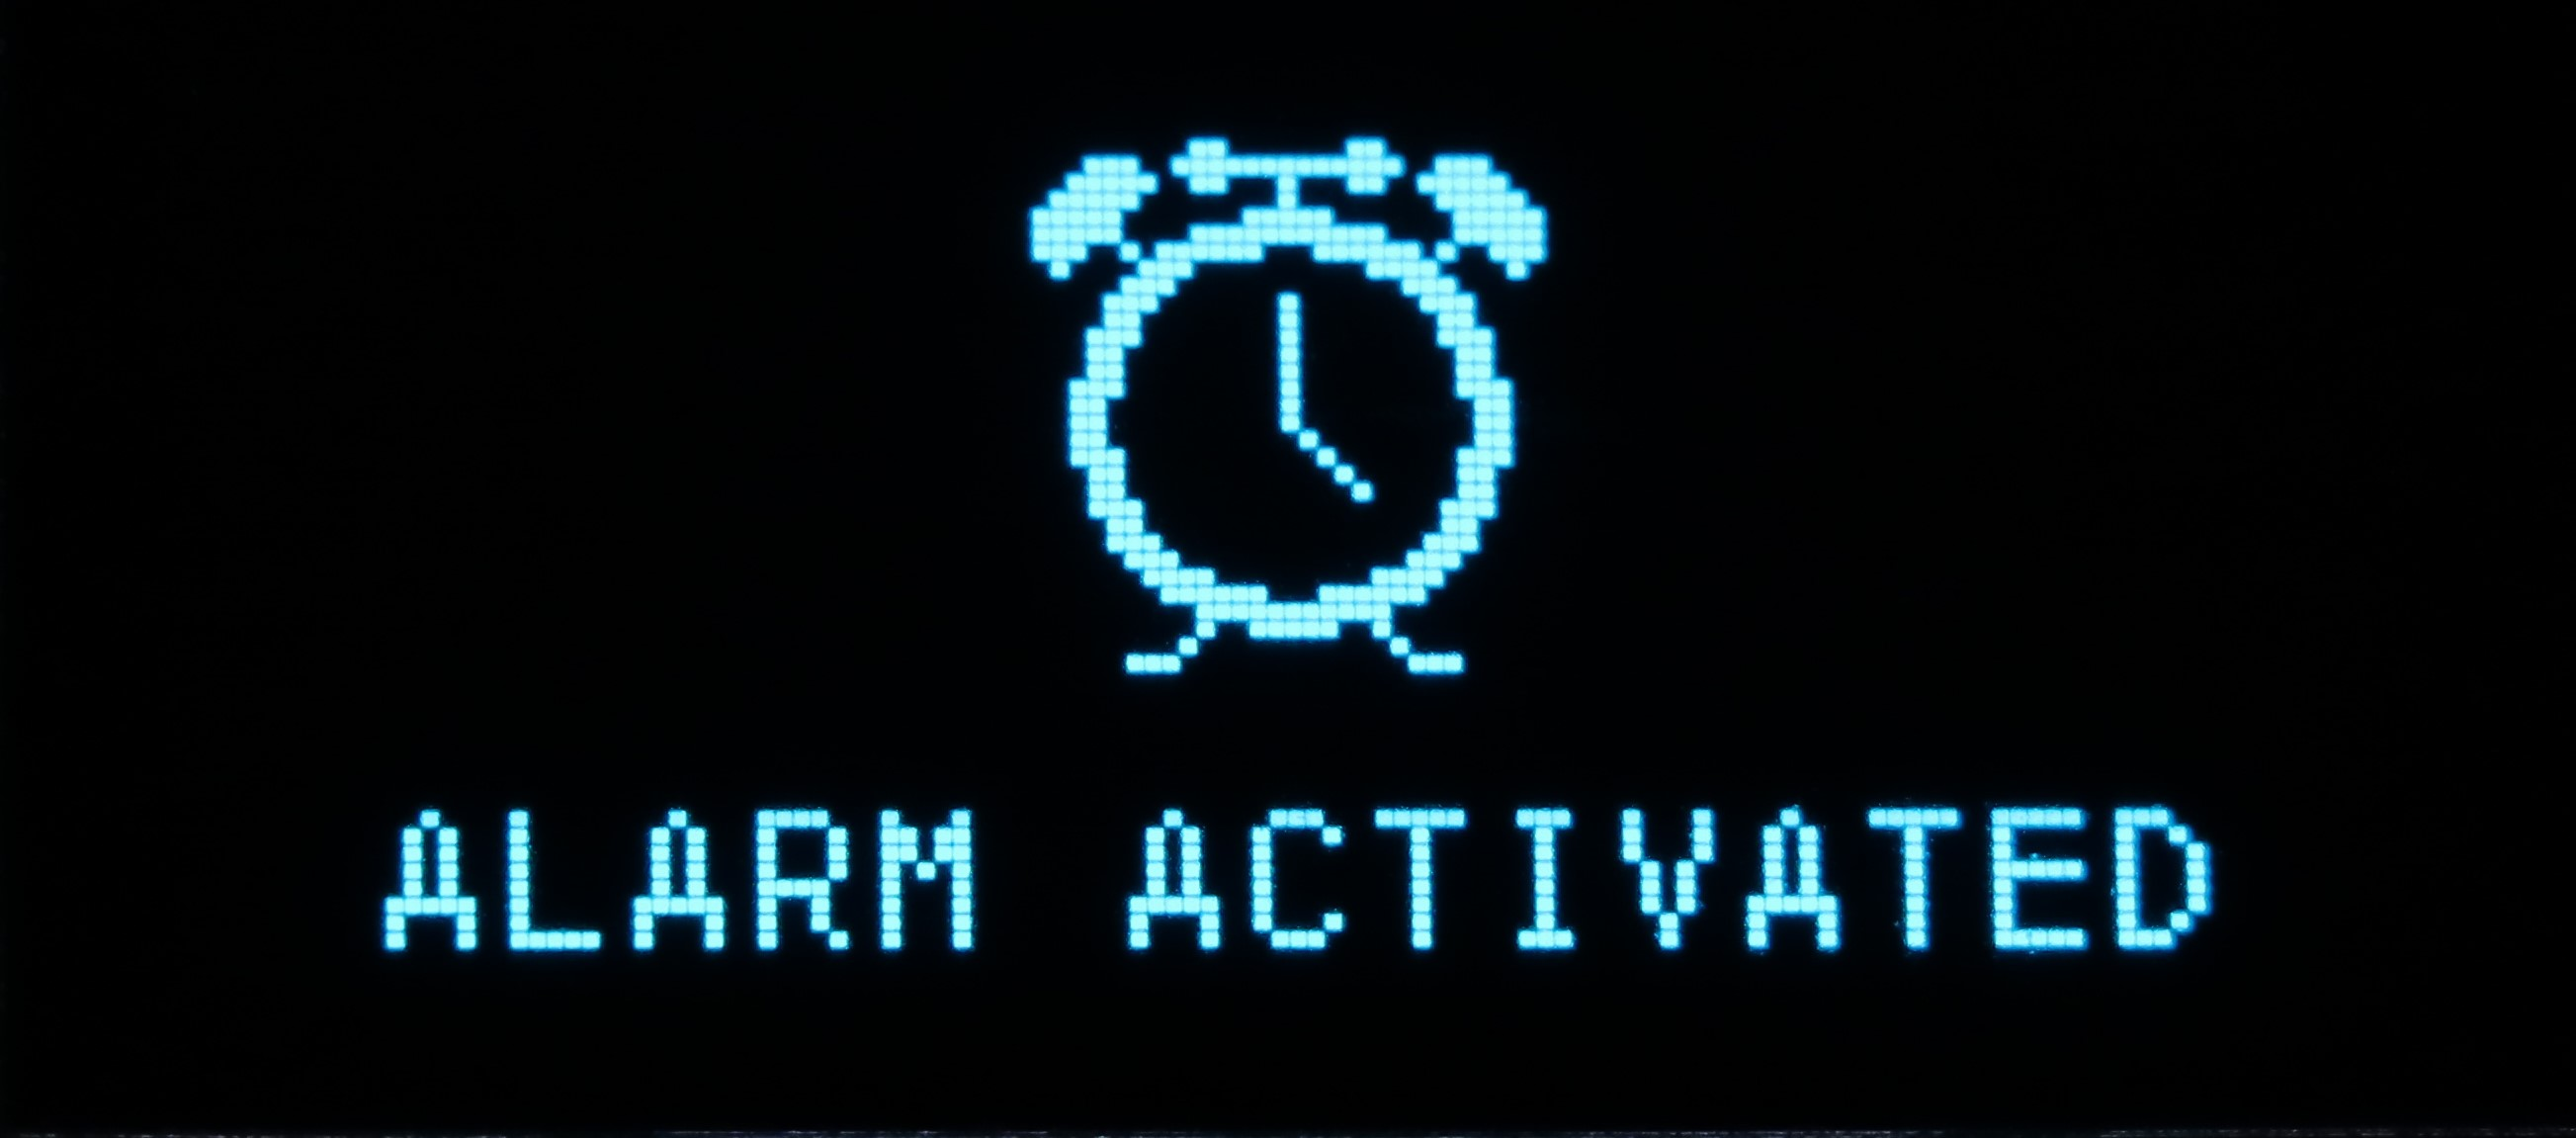
\includegraphics[width=0.5\linewidth]{state_alarm}
		\caption{صفحه‌ی آلارم}
		\label{fig:state-ringing}
	\end{figure}

تمامی اشکال موجود در صفحات پیکسل به پیکسل طراحی شده و از هیچ شکل آماده‌ای در این پروژه استفاده نشده است.
\newpage
\subsection{وقفه‌ها}
منابع وقفه در این پروژه 5 چیز است:
\begin{enumerate}
	\item وقفه‌ی خارجی\footnote{\lr{EXTI (External Interupt)}}:
	همانطور که در بخش \ref{sec:gpio} بحث شد، 5 پایه از پایه‌های \lr{GPIO} برای فعالسازی وقفه‌ی خارجی هستند:
	\begin{enumerate}
		\item کلیدهای لمسی:
		بعد از فعال شدن وقفه، با توجه به اینکه سیستم در چه حالتی از حالت‌های هفتگانه قرار دارد، توابع مشخصی اجرا می‌شوند. شرح کامل این اقدامات در بخش \ref{sec:fsm} داده شده است. شکل \ref{fig:exti} یک نمونه از این کدها را نشان می‌دهد.
		\begin{figure}[h]
			\centering
			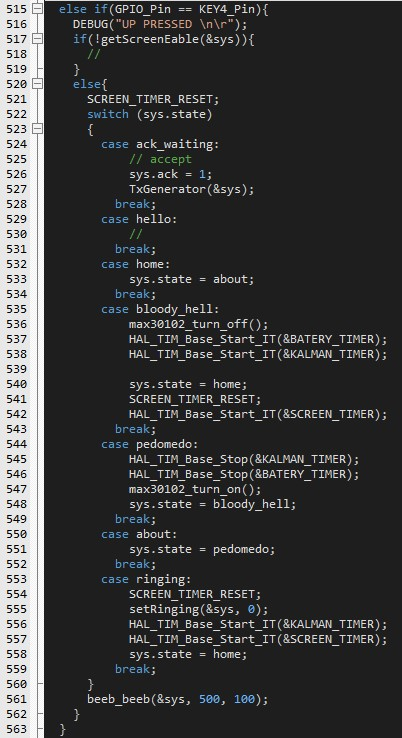
\includegraphics[width=0.55\linewidth]{exti}
			\caption{نمونه کدی از بخش وقفه‌ی خارحی}
			\label{fig:exti}
		\end{figure}
	
		\item وقفه‌ی حسگر \lr{PPG}: هنگامی که حسگر داده‌ی جدیدی داشته باشد، با فعال کردن یک پایه، وقفه‌ای را فعال می‌کند. در روتین این وقفه داده‌های حسگر قرائت می‌شود و به ترتیب در یک آرایه ذخیره می‌شوند. هنگامی که این آرایه پر شود، توسط بلوتوث به گوشی ارسال می‌گردد. شکل \ref{fig:exti-ppg} بخش مربوط به ذخیره در آرایه و ارسال آن را نشان می‌دهد.
		\begin{figure}[h]
			\centering
			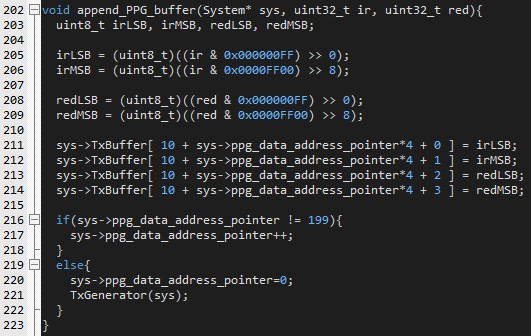
\includegraphics[width=0.7\linewidth]{exti_ppg}
			\caption{نمونه کدی از بخش ذخیره‌ی داده‌ی حسگر سلامت}
			\label{fig:exti-ppg}
		\end{figure}
		
	\end{enumerate}
	\item وقفه‌ی تایمر:
	همانطور که گفته شد سه تایمر از هفت تایمر برای فعالسازی وقفه به کار رفته‌اند:
	\begin{enumerate}
		\item تایمر فیلتر کالمن:
		این تایمر هر یک میلی ثانیه وقفه را فعال می‌کند. در روتین وقفه ابتدا اطلاعات حسگر حرکتی خوانده می‌شود. سپس این اطلاعات برای فیلتر شدن به توابع کالمن داده می‌شود. شرج این توابع در بخش‌هایی بعدی آورده شده است. سپس اطلاعات فیلتر شده وارد مرحله‌ی پردازش می‌شوند. این پردازش‌ها شامل تشخیص سرعت زاویه‌ای دست حول آرنج و تشخیص گام است. کد این بخش در شکل \ref{fig:kalman-code} قابل مشاهده است.
		\begin{figure}[h]
			\centering
			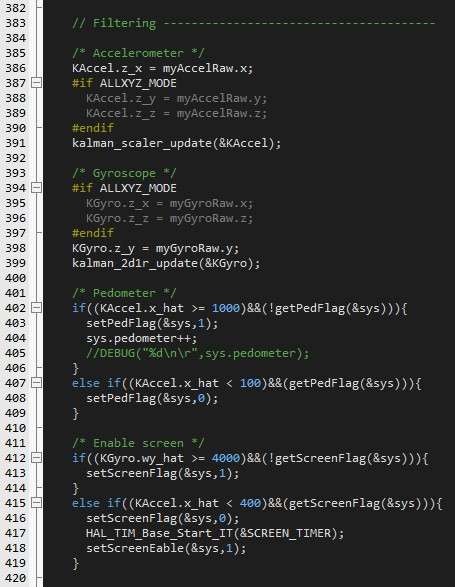
\includegraphics[width=0.5\linewidth]{kalman_code}
			\caption{نمونه کدی از بخش وقفه‌ی کالمن}
			\label{fig:kalman-code}
		\end{figure}
		
		\item تایمر صفحه نمایش:
		هرگاه وقفه‌ی این تایمر فعال شود به این معنی است که چهار ثانیه از آخرین تعامل کاربر با ساعت گذشته است و باید صفحه نمایش خاموش شود. شکل \ref{fig:screen-timer} کد این قسمت را نشان می‌دهد.
		\begin{figure}[h]
			\centering
			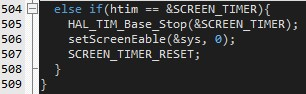
\includegraphics[width=0.5\linewidth]{screen_timer}
			\caption{کد روتین وقفه‌ی تایمر صفحه نمایش}
			\label{fig:screen-timer}
		\end{figure}
		
		\item تایمر اصلی سیستم:
این تایمر هر 250 میلی ثانیه سرریز می‌شود. در نتیجه هر 250 میلی ثانیه روتین وقفه اجرا می‌شود. در روتین وقفه‌ی این تایمر ابتدا بررسی می‌شود که آیا صفحه نمایش باید روشن شود یا خیر. اگر نیاز به روشن شدن بود، با توجه به حالت سیستم و ماشین حالتی که در بخش \ref{sec:fsm} توضیح داده شد، روتین حالت مربوطه را اجرا می‌کند.
	\end{enumerate}
	\item وقفه‌ی آلارم:
	هنگامی که ساعت و روز بر ساعت و روز آلارم منطبق شود، این وقفه فعال می‌گردد. در روتین این وقفه پرچم آلارم یک می‌شود، تایمر کالمن خاموش می‌شود، صفحه نمایش روشن می‌شود و حالت سیستم به آلارم تغییر می‌کند.
	\item وقفه‌ی \lr{DMA} مربوطه به \lr{ADC}:
	تنظیمات \lr{DMA} مربوط به \lr{ADC} به گونه‌ای است که \lr{ADC} هر 10 میلی ثانیه یک نمونه می‌گیرد و آن را در آرایه‌ای ذخیره می‌کند. هرگاه این آرایه که طول آن 128 است پر شود، این وقفه فعال می‌شود. در روتین وقفه می‌خواهیم میانگین این 128 نمونه را به عنوان عدد نهایی گزارش کنیم. میانگین ساده‌ترین راه جلوگیری از ورود نویز به سیستم است.
	
	پس مطابق شکل \ref{fig:adc-dma} ابتدا مجموع این 128 داده را حساب می‌کنیم. سپس باید این حاصل را بر تعداد نمونه‌ها تقسیم کنیم. فلسفه‌ی انتخاب عدد 128 برای تعداد نمونه‌ها اینجا مشخص می‌شود. می‌دانیم تقسیمات اعشاری به دلیل پیچیدگی‌های محاسباتی، مقداری زیادی از حافظه را اشغال می‌کنند و سرعت کمتری دارند. پس بهتر است تا جای ممکن از آن‌ها دوری کنیم.
	
	از طرفی می‌دانیم که اگر مقسوم‌علیه توان دو باشد، می‌توان عملیات تقسیم را با شیفت مقسوم انجام داد. در اینجا جای اینکه مجموع را بر 128 تقسیم کنیم، کافی است آن را 7 بیت به سمت راست شیفت دهیم تا تقسیم انجام شود. اینگونه هم سرعت بسیار بالایی دارد هم حافظه را بیهوده اشغال نمی‌کند.
	\begin{figure}[h]
		\centering
		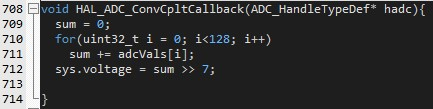
\includegraphics[width=0.5\linewidth]{adc_dma}
		\caption{کد روتین وقفه‌ی \lr{DMA} مربوطه به \lr{ADC}}
		\label{fig:adc-dma}
	\end{figure}
	\item وقفه‌ی \lr{DMA} مربوطه به \lr{UASRT}:
	تنظیمات \lr{DMA} مربوط به \lr{USART} به گونه‌ای است که هرگاه تعداد 21 بایت داده توسط واحد ارتباط سریال (بلوتوث) دریافت شود، وقفه‌ی مربوطه فعال می‌‌شود. در روتین این وقفه این داده تحلیل می‌شود و بسته به نوع آن، اقدام مناسب با آن صورت می‌گیرد. جزئیات مربوط به بسته‌ها و نحوه‌ی کدگشایی آن‌ها در بخش \ref{sec:comm} توضیح داده خواهد شد.
\end{enumerate}
\subsection{لایه‌های نرم‌افزاری}
ساختار کد به صورت لایه‌ای است. به این معنی که هر قطعه کد یا کتابخانه از توابع موجود در کتابخانه‌های لایه‌ی پایین استفاده می‌کند. شکل \ref{fig:sfarch} نحوه‌ی لایه‌بندی این پروژه را نشان می‌دهد.
\begin{figure}[h]
	\centering
	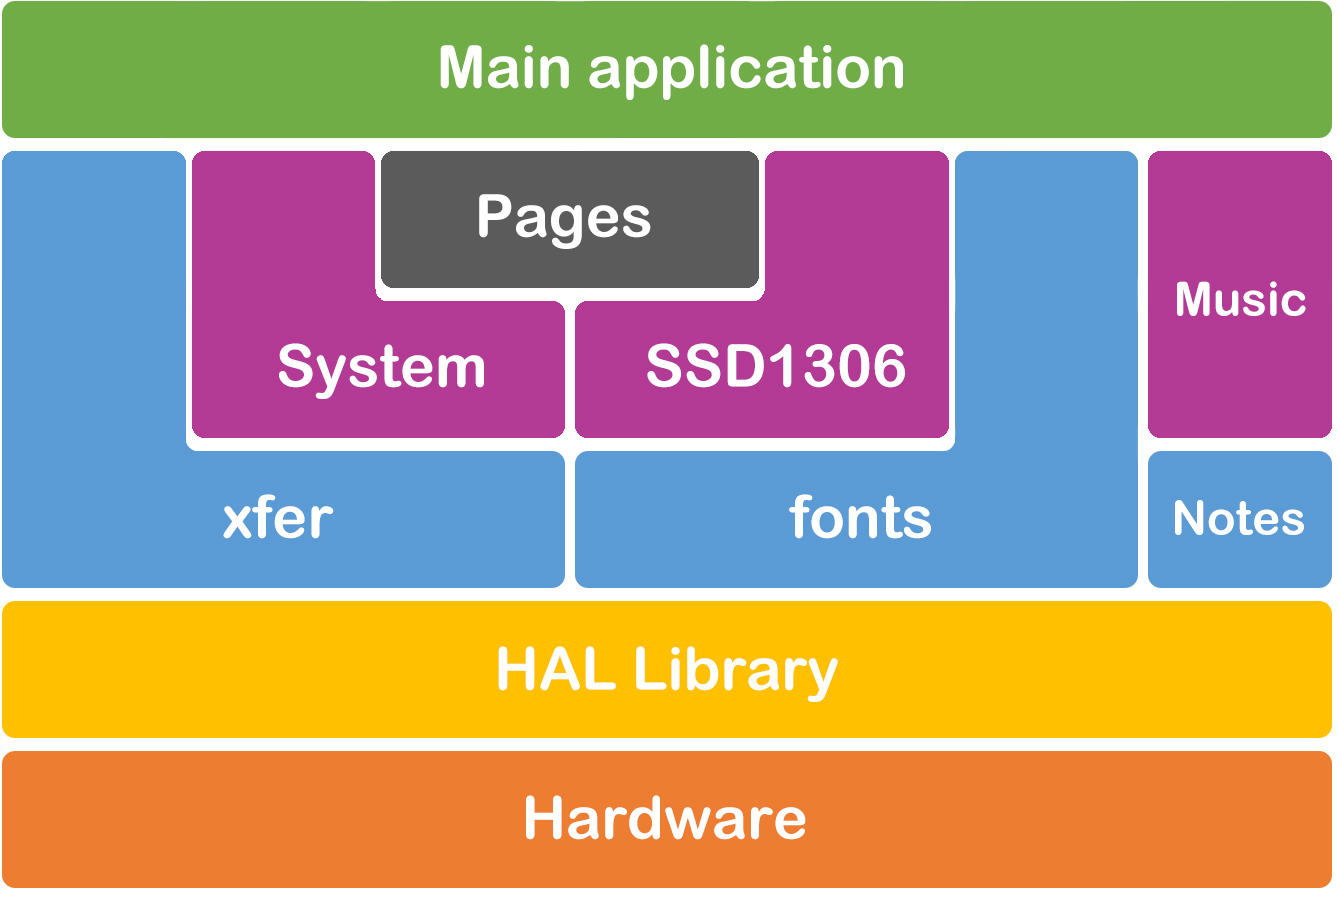
\includegraphics[width=0.8\linewidth]{sfarch}
	\caption{لایه‌های نرم‌افزاری}
	\label{fig:sfarch}
\end{figure}

پایین‌ترین لایه، لایه‌ی سخت‌افزار است. رجیسترهایی که برای کار با سخت‌افزار مورد نیاز است در این لایه قرار دارد. از آنجا کار با رجیسترها به صورت مستقیم اگرچه در مواردی بهتر و بهینه‌تر است، اما دشواری‌هایی دارد که در اکثر موارد مانع استفاده از آن می‌شود. این پروژه نیز از این قاعده مستثنی نیست. برای ساده کردن کار با سخت‌افزار، از یک کتابخانه به نام
\lr{HAL}\footnote{\lr{Hardware Abstraction Layer}}
بهره بردیم که به کمک توابع موجود در آن کار با سخت‌افزار ساده می‌شود. بقیه‌ی لایه‌ها روی لایه‌ی \lr{HAL} سوار می‌شوند.

دیگر لایه‌ها شامل کتابخانه‌هایی است که برای بخش‌های مختلف پروژه نوشته شده است. در ادامه به صورت کلی به توضیح این کتابخانه‌ها پرداخته می‌شود.

\subsubsection{کتابخانه‌ی \lr{xfer}}
این کتابخانه شامل دو تابع است که وظیفه‌ی ارسال داده‌ها از طریق سخت‌افزار را برعهده دارند. تصویر این توابع در شکل \ref{fig:xfer} دیده می‌شود.

\begin{figure}[h]
	\centering
	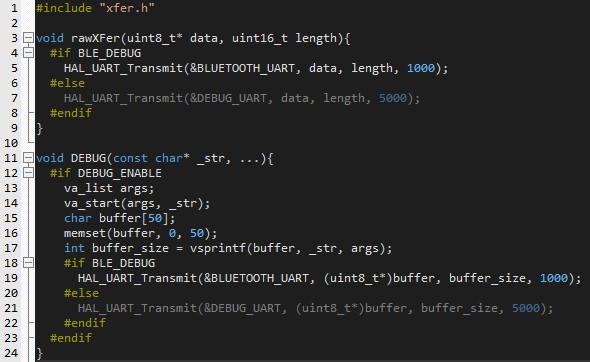
\includegraphics[width=0.8\linewidth]{xfer}
	\caption{توابع کتابخانه‌ی \lr{xfer}}
	\label{fig:xfer}
\end{figure}

\subsubsection{کتابخانه‌ی \lr{fonts}}
این کتابخانه شامل فونت‌ها و اشکالی است که روی صفحه نمایش نشان داده خواهند شد. تصویر بخشی از این کدها در شکل \ref{fig:fonts} دیده می‌شود.

\begin{figure}[h]
	\centering
	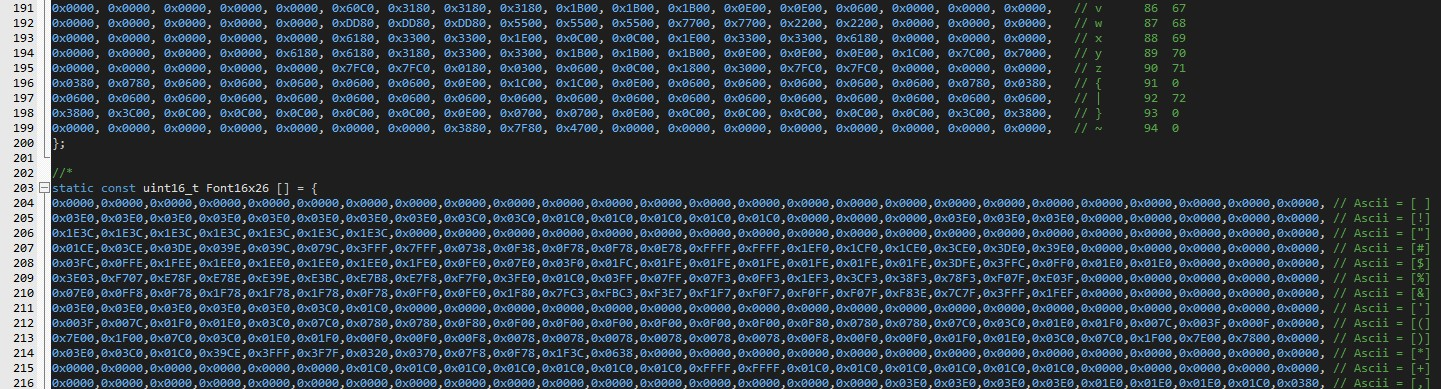
\includegraphics[width=\linewidth]{fonts}
	\caption{بخشی از کتابخانه‌ی \lr{fonts}}
	\label{fig:fonts}
\end{figure}

\newpage
\subsubsection{کتابخانه‌ی \lr{notes}}
این کتابخانه شامل نگاشتی از نت‌های موسیقی به فرکانس آن ها است. تصویر بخشی از این کدها در شکل \ref{fig:notes} دیده می‌شود.

\begin{figure}[h]
	\centering
	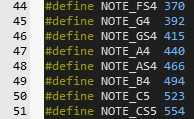
\includegraphics[width=0.3\linewidth]{notes}
	\caption{بخشی از کتابخانه‌ی \lr{notes}}
	\label{fig:notes}
\end{figure}

\subsubsection{کتابخانه‌ی \lr{max30102}}
این کتابخانه برای کار با حسگر \lr{PPG} است که توسط آقای \lr{Pan} نوشته شده است \cite{max30102}. شکل \ref{fig:max} نام توابع موجود در این کتابخانه را نشان می‌دهد.

\begin{figure}[h]
	\centering
	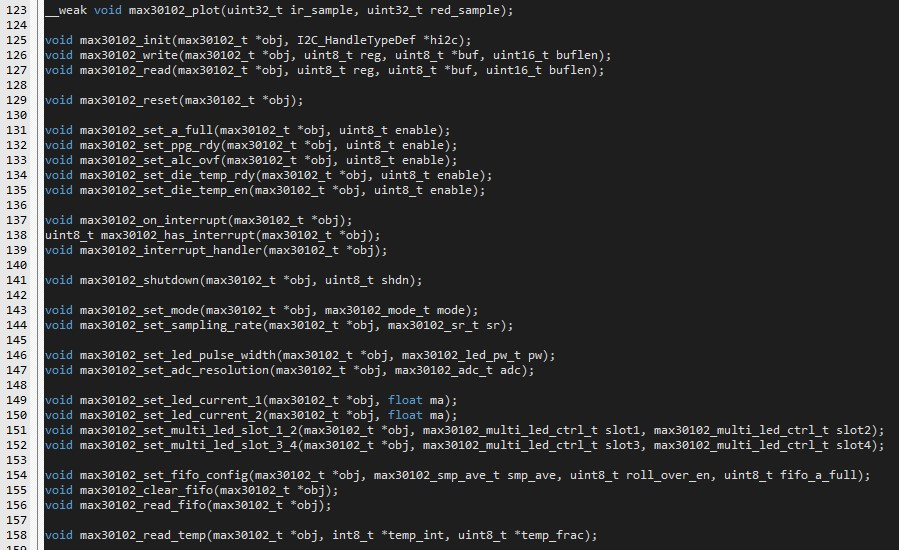
\includegraphics[width=\linewidth]{max30102}
	\caption{پروتوتایپ توابع کتابخانه‌ی \lr{MAX30102}}
	\label{fig:max}
\end{figure}

\newpage
\subsubsection{کتابخانه‌ی \lr{MPU6050}}
این کتابخانه برای کار با حسگر \lr{MPU6050} است که توسط آقای محمد یعقوب نوشته شده است \cite{mpu6050}. شکل \ref{fig:mpu} نام توابع موجود در این کتابخانه را نشان می‌دهد.

\begin{figure}[h]
	\centering
	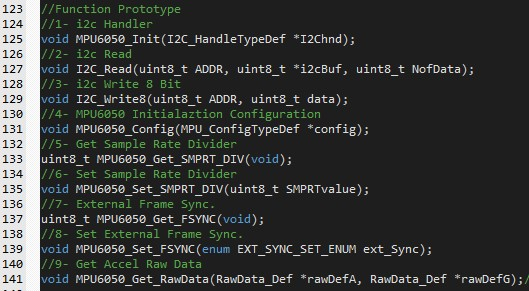
\includegraphics[width=0.6\linewidth]{mpu6050}
	\caption{پروتوتایپ توابع کتابخانه‌ی \lr{MPU6050}}
	\label{fig:mpu}
\end{figure}

\subsubsection{کتابخانه‌ی \lr{music}}
در این کتابخانه موسیقی «ای ایران ای مرز پرگهر» به صورت نت‌های موسیقی نوشته شده است تا هنگام فعال شدن آلارم نواخته شود. شکل \ref{fig:music} این نت‌ها را نشان می‌دهد.

\begin{figure}[h]
	\centering
	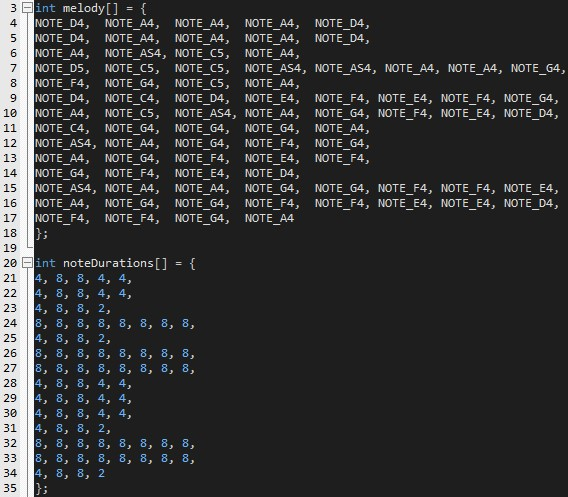
\includegraphics[width=0.7\linewidth]{eyiran}
	\caption{نت‌های «ای ایران»}
	\label{fig:music}
\end{figure}

\subsubsection{کتابخانه‌ی \lr{SSD1306}}
این کتابخانه برای کار با صفحه نمایش‌های با درایور \lr{SSD1306} است که توسط آقای \lr{Olivier Van den Eede} نوشته شده است \cite{ssd1306}. شکل \ref{fig:ssd1306} نام توابع موجود در این کتابخانه را نشان می‌دهد.

\begin{figure}[h]
	\centering
	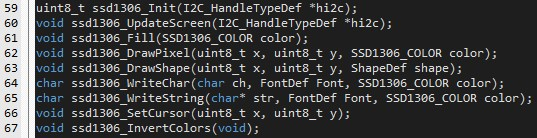
\includegraphics[width=0.8\linewidth]{ssd1306}
	\caption{پروتوتایپ توابع کتابخانه‌ی \lr{SSD1306}}
	\label{fig:ssd1306}
\end{figure}

\subsubsection{کتابخانه‌ی \lr{Kalman}}
در این کتابخانه توابع و روابط فیلتر کالمن پیاده‌سازی شده است. توضیحات مفصل این توابع در بخش \ref{sec:kalman} داده خواهد شد. شکل \ref{fig:kalman} نام توابع موجود در این کتابخانه را نشان می‌دهد.

\begin{figure}[h]
	\centering
	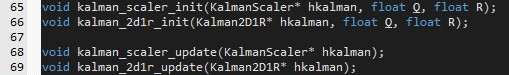
\includegraphics[width=0.8\linewidth]{kalman}
	\caption{پروتوتایپ توابع کتابخانه‌ی \lr{kalman}}
	\label{fig:kalman}
\end{figure}

\subsubsection{کتابخانه‌ی \lr{Pages}}
در این کتابخانه توابعی که بسته به حالت سیستم، صفحه‌ی مورد نظر را روی صفحه نمایش ترسیم می‌کنند. شکل \ref{fig:pages} نام توابع موجود در این کتابخانه را نشان می‌دهد.

\begin{figure}[h]
	\centering
	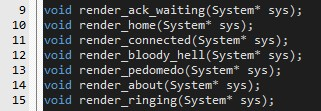
\includegraphics[width=0.6\linewidth]{pages}
	\caption{پروتوتایپ توابع کتابخانه‌ی \lr{pages}}
	\label{fig:pages}
\end{figure}

\subsubsection{کتابخانه‌ی \lr{System}}
می‌توان گفت این کتابخانه حیاتی‌ترین کتابخانه است. در این کتابخانه توابع مربوط به سیستم قرار دارد. همچنین یک ساختار\footnote{\lr{Struct}}
تعریف شده تا متغیرهای سیستمی را شامل شود. شکل \ref{fig:system} نام توابع موجود در این کتابخانه و شکل \ref{fig:system_struct} تعریف این ساختار را نشان می‌دهد.

\begin{figure}[h]
	\centering
	\begin{subfigure}{0.95\textwidth}
		\centering
		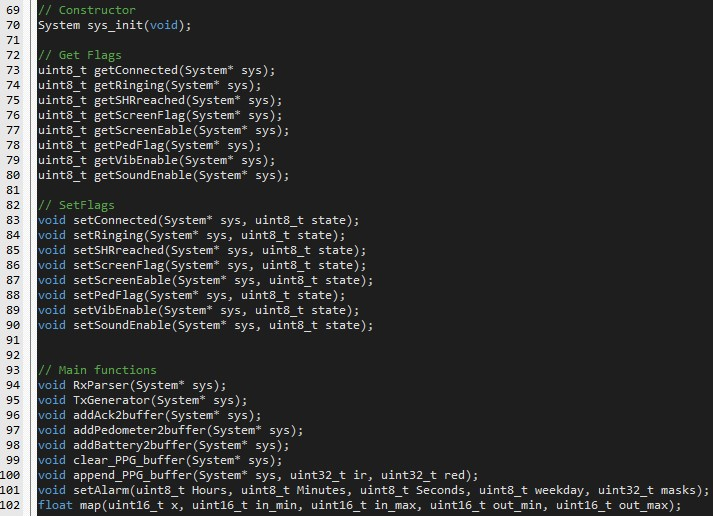
\includegraphics[width=0.8\linewidth]{system}
		\caption{پروتوتایپ توابع کتابخانه‌ی \lr{system}}
		\label{fig:system}
	\end{subfigure} \\
	\begin{subfigure}{0.95\textwidth}
		\centering
		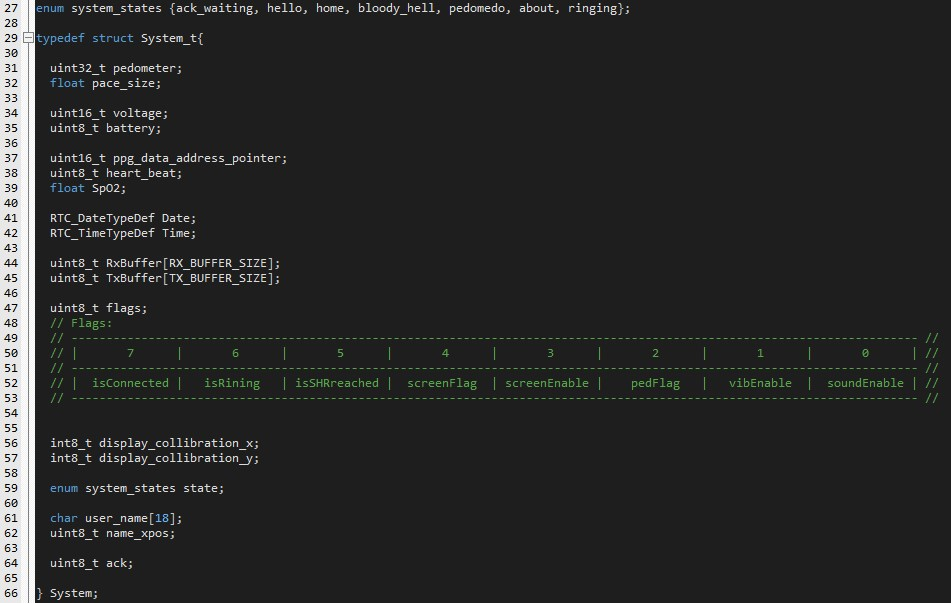
\includegraphics[width=0.8\linewidth]{system_struct}
		\caption{متغیرهای \lr{struct} سیستم}
		\label{fig:system_struct}
	\end{subfigure}
	\caption{تصاویر مربوطه به کتابخانه‌ی \lr{system}}
\end{figure}

\section{پردازش داده‌های حسگر حرکتی} \label{sec:kalman}
دو مورد از وظایفی که برای ساعت تعریف شده است، شمردن تعداد گام‌ها و روشن کردن صفحه نمایش در صورت بالا آمدن دست است. برای انجام این وظایف از حسگر حرکتی \lr{MPU6050} استفاده شده است. اما می‌دانیم ادوات اندازه‌گیری دارای نویز و نایقینی‌های مختلف هستند. حسگر فوق نیز از این قاعده مستثنی نیست. لذا قبل از هر چیز باید داده‌ی آن فیلتر شود تا نویز و اثرات مخرب دیگر تا جای ممکن بر پردازش‌ها اثر نگذارند. به این منظور یک فیلتر کالمن طراحی و پیاده‌سازی شده است. شکل \ref{fig:kalman-block} بلوک دیاگرام زیر سیستم تشخیص حرکت را نشان می‌دهد.

\begin{figure}[h]
	\centering
	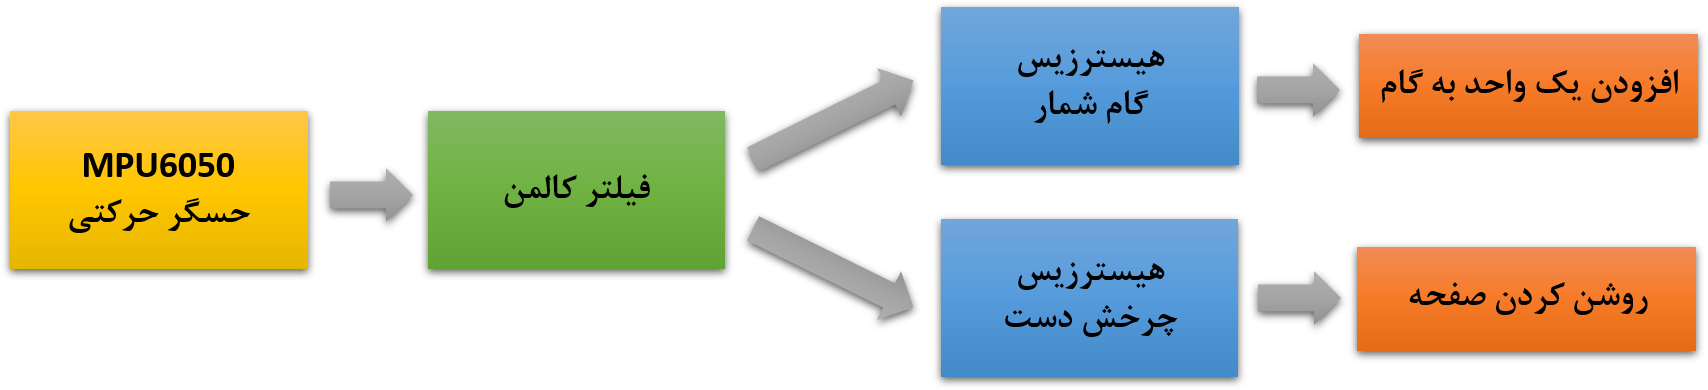
\includegraphics[width=\linewidth]{kalman_block}
	\caption{بلوک دیاگرام زیر سیستم تشخیص حرکت}
	\label{fig:kalman-block}
\end{figure}

برای طراحی بلوک دیاگرام فوق، ابتدا نویز حسگر را بشناسیم. بدین منظور چند ثانیه از داده‌های حسگر توسط ساعت نمونه‌برداری شد و توسط بلوتوث به نرم‌افزار متلب ارسال شد. این نمونه‌ها به مدت یازده ثانیه ضبط شدند. در این مدت حرکات تصادفی و متنوعی را به ساعت اعمال کردم. شکل \ref{fig:mpu-raw} خروجی حسگر را در این مدت نشان می‌دهد.

\begin{figure}[h]
	\centering
	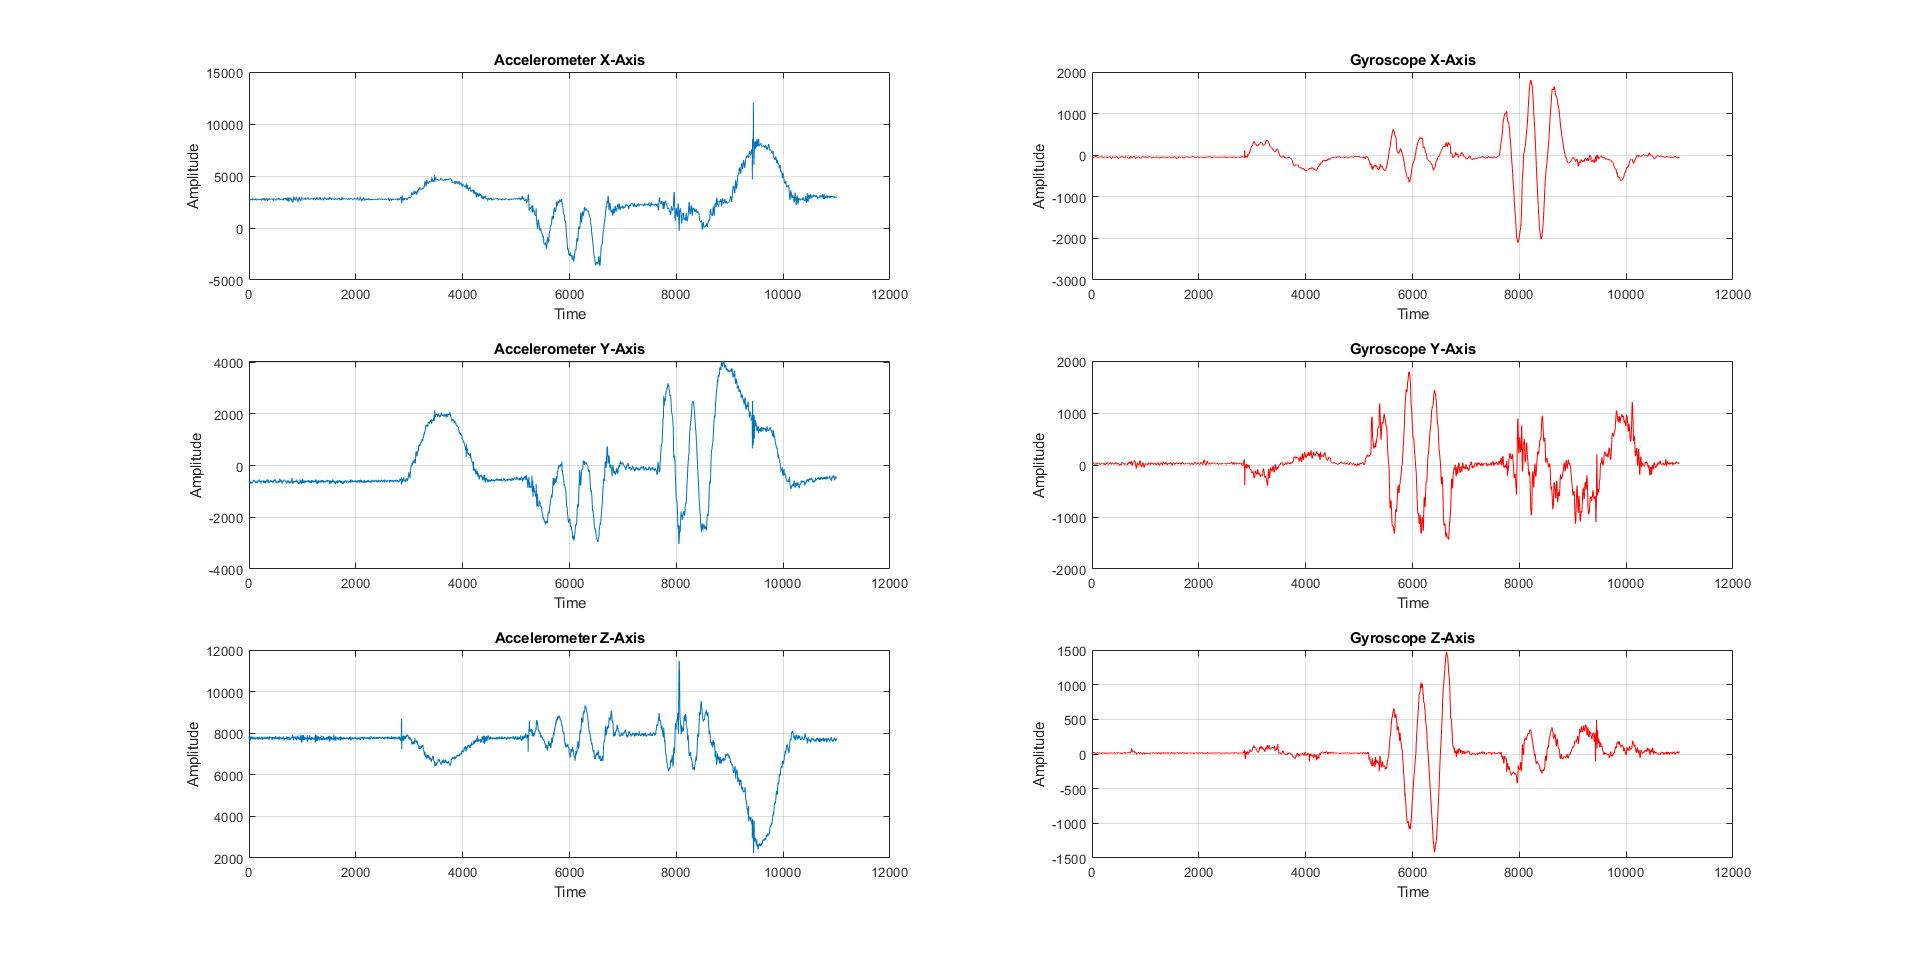
\includegraphics[width=\linewidth]{mpu_raw}
	\caption{خروجی حسگر حرکتی. سه محور مربوط به شتاب خطی و سه محور مربوط به سرعت زاویه‌ای}
	\label{fig:mpu-raw}
\end{figure}

همانطور که در خروجی حسگر مشهود است، مقدار نویز قابل توجه است و می‌تواند پردازش‌ها را دچار خطا کند. از این رو به طراحی فیلتر کالمن می‌پردازیم.

\subsection{فیلتر کالمن}
گام اول طراحی فیلتر کالمن، مدلسازی سیستم است. حسگر حرکتی سیستمی است کنترل نشده. لذا حلقه‌ی کنترلی‌ای در کار نیست. می‌توان گفت ورودی این حسگر شتاب حرکت دست است. در نتیجه سیستم شتاب سنج حسگر را می‌توان به صورت معادله‌ی \ref{eq:linmove} مدل کرد که در آن $x$ موقعیت، $v$ سرعت خطی، $a$ شتاب خطی و $T$ فاصله‌ی زمانی دو نمونه یا همان تناوب نمونه‌برداری یا گسسته‌سازی است.
\begin{equation}
	x[n+1] = \frac{1}{2}a[n]T^2 + v[n]T + x[n] 
	\label{eq:linmove}
\end{equation}

سیستم سرعت زاویه‌ای نیز به طور مشابه به صورت معادله‌ی \ref{eq:rotmove} مدل می‌شود که در آن $\theta$ زاویه، $\omega$ سرعت زاویه‌ای، $\alpha$ شتاب زاویه‌ای و $T$ فاصله‌ی زمانی دو نمونه یا همان تناوب نمونه‌برداری یا گسسته‌سازی است.
\begin{equation}
	\theta[n+1] = \frac{1}{2}\alpha[n]T^2 + \omega[n]T + \theta[n] 
	\label{eq:rotmove}
\end{equation}

از آنجا که حرکت دست، یا به عبارتی تغییرات شتاب خطی/زاویه‌ای نامشخص است، می‌توان آن را به صورت اغتشاش ورودی مدل کرد. در نتیجه تغییرات شتاب اغتشاشی است که به سیستم وارد می‌شود تا متغیرهای سیستم (موقعیت و سرعت) را تغییر دهد. بنابراین می‌توان فرم فضای حالت را برای این سیستم‌ها به صورت معادلات \ref{eq:sslin} و \ref{eq:ssrot} نوشت:

\begin{gather}
	\begin{bmatrix}
		x[n+1] \\
		v[n+1] \\
		a[n+1]
	\end{bmatrix}
	=
	\begin{bmatrix}
		1 & T & \frac{1}{2}T^2 \\
		0 & 1 & T \\
		0 & 0 & 1
	\end{bmatrix}
	\begin{bmatrix}
		x[n] \\
		v[n] \\
		a[n]
	\end{bmatrix}
	+
	\begin{bmatrix}
		0 \\
		0 \\
		1
	\end{bmatrix}
	w_{linear}[n]
	\label{eq:sslin} \\
	\begin{bmatrix}
		\theta[n+1] \\
		\omega[n+1] \\
		\alpha[n+1]
	\end{bmatrix}
	=
	\begin{bmatrix}
		1 & T & \frac{1}{2}T^2 \\
		0 & 1 & T \\
		0 & 0 & 1
	\end{bmatrix}
	\begin{bmatrix}
		\theta[n] \\
		\omega[n] \\
		\alpha[n]
	\end{bmatrix}
	+
	\begin{bmatrix}
		0 \\
		0 \\
		1
	\end{bmatrix}
	w_{rotational}[n]
	\label{eq:ssrot}
\end{gather}

گام دوم مدلسازی مشاهده از حالت‌های سیستم است. همانطور که از معادلات فوق مشخص است، ماتریس‌های حالت ($\phi$) و ورودی ($G$) در هر دو حالت خطی و زاویه‌ای یکسان هستند و می‌توان مدل یکسانی به هر دو حرکت نسبت داد. اما از طرفی می‌دانیم که خروجی حسگر برای حالت خطی، شتاب و برای حالت زاویه‌ای، سرعت است. در نتیجه معادلات استاتیکی مشاهده به شکل معادلات \ref{eq:zlin} و \ref{eq:zrot} خواهند بود.

\begin{gather}
	z_{linear} = 
	\begin{bmatrix}
		0 & 0 & 1
	\end{bmatrix}
	\begin{bmatrix}
		x \\
		v \\
		a
	\end{bmatrix}
	+ v_{linear} 
	\label{eq:zlin} \\
	z_{rotational} = 
	\begin{bmatrix}
		0 & 1 & 0
	\end{bmatrix}
	\begin{bmatrix}
		\theta \\
		\omega \\
		\alpha
	\end{bmatrix}
	+ v_{rotational} 
	\label{eq:zrot}
\end{gather}


نکته‌ی مهمی در رابطه با حسگر سرعت زاویه‌ای وجود دارد. حسگرهای
\lr{MEMS}\footnote{\lr{Micro-ElectroMechanical Systems}}
که برای اندازه‌گیری سرعت زاویه‌ای استفاده می‌شوند، بخاطر ساختارشان یک عبارت نامشخص ولی ثابت\footnote{\lr{Bias}} را در خروجی با مقدار واقعی جمع می‌کنند. این عبارت بایاس را می‌توان به عنوان یک حالت جدید به مدل سیستم افزود. در این حالت مدل نهایی به صورت معادلات \ref{eq:ssrot-bias} و \ref{eq:zrot-bias} خواهد بود.

\begin{gather}
	\begin{bmatrix}
		\theta[n+1] \\
		\omega[n+1] \\
		\alpha[n+1] \\
		b[n+1]
	\end{bmatrix}
	=
	\begin{bmatrix}
		1 & T & \frac{1}{2}T^2 & 0\\
		0 & 1 & T & 0\\
		0 & 0 & 1 & 0 \\
		0 & 0 & 0 & 1
	\end{bmatrix}
	\begin{bmatrix}
		\theta[n] \\
		\omega[n] \\
		\alpha[n] \\
		b[n]
	\end{bmatrix}
	+
	\begin{bmatrix}
		0 \\
		0 \\
		1 \\
		0
	\end{bmatrix}
	w_{rotational}[n]
	\label{eq:ssrot-bias} \\
	z_{rotational} = 
	\begin{bmatrix}
		0 & 1 & 0 & 1
	\end{bmatrix}
	\begin{bmatrix}
		\theta \\
		\omega \\
		\alpha \\
		b
	\end{bmatrix}
	+ v_{rotational} 
	\label{eq:zrot-bias}
\end{gather}

در این پروژه لازم است تا صرفا الگوی «کلی» تغییرات شتاب خطی و الگوی «کلی» تغییرات سرعت زاویه‌ای مورد بررسی قرار گیرند. از این رو فرض‌های ذیل معقول‌اند:
\begin{enumerate}
	\item عبارت بایاس مقدار کوچکی است؛ از طرفی تأثیری نیز در الگوی تغییرات ندارد لذا می‌توان از آن صرف‌نظر کرد.
	\item در تحلیل حرکت خطی، نیازی به تخمین موقعیت و سرعت نیست و صرفا شتاب اهمیت دارد، لذا می‌توان حالت‌های موقعیت و سرعت را از معادله‌ی حالت حذف کرد.
	\item در تحیل حرکت دورانی نیازی به تخمین زاویه نیست و صرفا سرعت زاویه‌ای اهمیت دارد. لذا می‌توان حالت زاویه را از معادله‌ی حالت حذف کرد.
	\item چون  صرفا الگوی سیگنال اهمیت دارد، نیازی به تبدیل واحد به واحدهای استاندارد نیست.
\end{enumerate}

\newpage
با اعمال مفروضات فوق، معادلات حرکت خطی به شکل معادله‌ی \ref{eq:lin-final} و معادلات حرکت دورانی به شکل معادله‌ی \ref{eq:rot-final} در می‌آیند.

\begin{gather}
	a[n+1] = a[n] + w_{linear}[n] \nonumber
	\\
	z_{rotational} = a + v_{linear} 
	\label{eq:lin-final}
\end{gather}
\begin{gather}
	\begin{bmatrix}
		\omega[n+1] \\
		\alpha[n+1] 
	\end{bmatrix}
	=
	\begin{bmatrix}
		1 & T \\
		0 & 1
	\end{bmatrix}
	\begin{bmatrix}
		\omega[n] \\
		\alpha[n]
	\end{bmatrix}
	+
	\begin{bmatrix}
		0 \\
		1
	\end{bmatrix}
	w_{rotational}[n] \nonumber
	\\
	z_{rotational} = 
	\begin{bmatrix}
		1 & 0
	\end{bmatrix}
	\begin{bmatrix}
		\omega \\
		\alpha
	\end{bmatrix}
	+ v_{rotational} 
	\label{eq:rot-final}
\end{gather}

گام سوم طراحی معادلات کالمن برای دو سیستم بالا است. معادلات کالمن در حالت کلی به صورت \ref{eq:kalan-main} است \cite{uncertain}.

\begin{gather}
	\hat{x}(N+1) = \phi(N)\hat{x}(N) + K(N)(z(N)-H(N)\phi(N)\hat{x}(N)) \nonumber \\
	K = \Sigma(N+1|N)H(N)^T(H(N)\Sigma(N+1|N)H(N)^T+R(N))^{-1} \nonumber \\
	\Sigma(N+1|N) = \phi(N)\Sigma(N|N)\phi(N)^T + G(N)Q(N)G(N)^T \nonumber \\
	\Sigma(N+1|N+1) = (I-K(N)H(N))\Sigma(N+1|N)(I-K(N)H(N))^T+K(N)R(N)K(N)^T \label{eq:kalan-main}
\end{gather}

از آنجا که ماتریس‌های دو سیستم متفاوت هستند، هرکدام مستلزم بکارگیری معادلات متفاوتی برای فیلتر شدن هستند. لذا هرکدام جداگانه شرح داده می‌شوند.
\begin{itemize}
	\item حرکت خطی: \\
از آنجا که معادلات حرکت خطی به صورت اسکالر درآمده‌اند و از طرفی سیستم نیز نامتغیر با زمان است، می‌توان ماتریس‌های سیستم را به صورت ذیل خلاصه کرد:
\begin{gather}
	\phi = 1 \quad,\quad G = 1\quad,\quad H = 1 \label{eq:linmat}
\end{gather}

\newpage
در صورتی که مقادیر \ref{eq:linmat} را در \ref{eq:kalan-main} جایگذاری کنیم، با کمی ساده‌سازی به معادلات \ref{eq:linkalman} می‌رسیم.

\begin{gather}
	\hat{a}[n+1] = \frac{R}{\Sigma(N|N)+Q+R} \hat{a}[n] + \frac{\Sigma(N|N)+Q}{\Sigma(N|N)+Q+R}z[n] \nonumber \\
	\Sigma(N+1|N+1) = \frac{(\Sigma(N|N)+Q)R}{\Sigma(N|N)+Q+R} \label{eq:linkalman}
\end{gather}

این معادلات برای پیاده‌سازی در ریزپردازنده مناسب‌اند و به راحتی اجزا می‌شوند.

	\item  حرکت دورانی: \\
سیستم حرکت دورانی یک سیستم مرتبه دوی نامتغیر با زمان است. لذا ماتریس‌های سیستم به صورت زیر خلاصه می‌شود:

\begin{gather}
	\phi = 
	\begin{bmatrix}
		1 & T \\
		0 & 1
	\end{bmatrix}
	\quad , \quad
	G = 
	\begin{bmatrix}
		0 \\
		1
	\end{bmatrix}
	\quad,\quad
	H = 
	\begin{bmatrix}
		1 & 0 \\
	\end{bmatrix}
	\label{eq:rotmat}
\end{gather}

\begin{figure}[h]
	\centering
	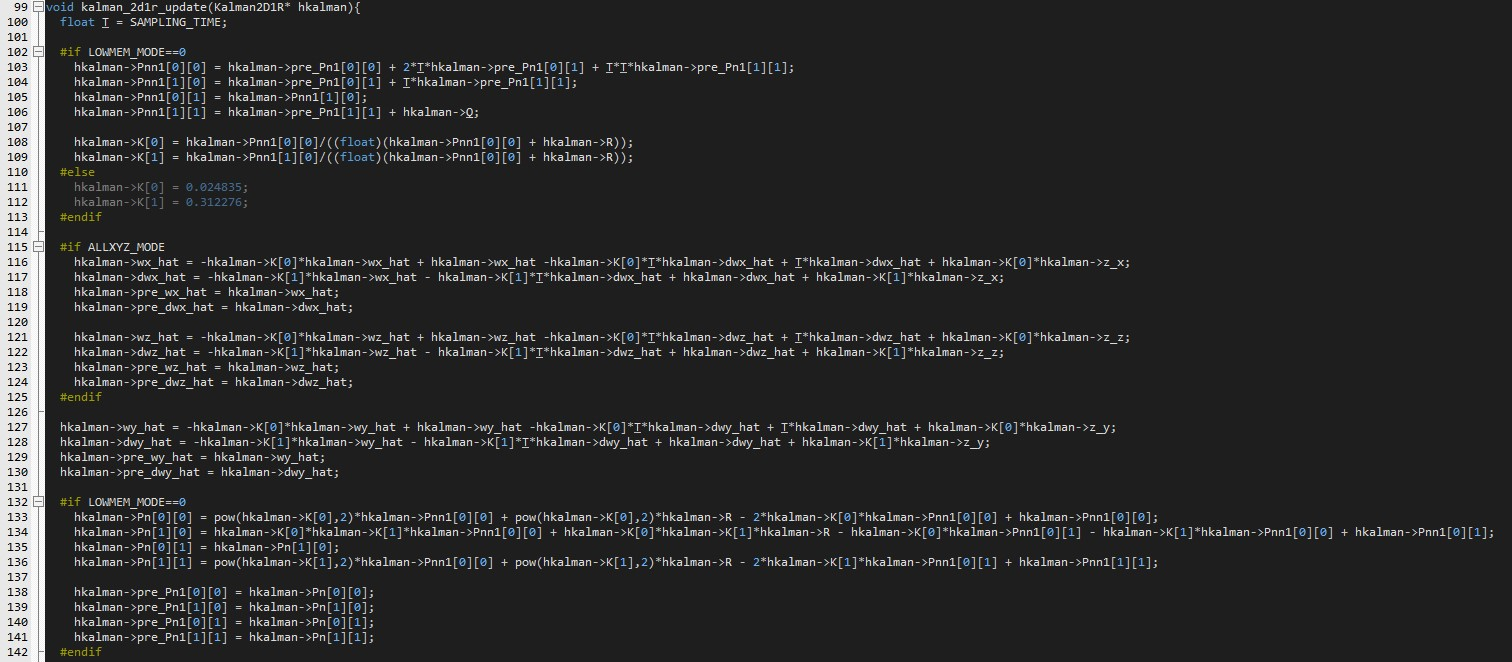
\includegraphics[width=\linewidth]{kalman_2d1r_codes}
	\caption{تصویر معادلات غیر ماتریسی کالمن به زبان \lr{C} برای سیستم حرکت دورانی}
	\label{fig:kalman-2d1r-code}
\end{figure}

جاگذاری \ref{eq:rotmat} در معادلات کالمن و محاسبه‌ی مقادیر تخمین زده شده کار ساده‌ای است. اما از آنجا که باید این محاسبات در ریزپردازنده اجرا شوند، دیگر امکان محاسبات ماتریسی به صورت عمومی وجود ندارد. زیرا مقدار حافظه و قدرت پردازشی بسیار محدود است. بدین جهت به کمک نرم‌افزار متلب و کتابخانه‌ی محاسبات سمبولیک آن، رابطه‌هایی که برای پیاده‌سازی به صورت غیرماترسی مورد نیاز است استخراج شد. این معادلات بسیار بزرگ هستند. لذا به تصویر این معادلات در برنامه بسنده می‌کنیم. شکل پیاده‌شده‌ی این معادلات در زبان \lr{C} به صورت شکل \ref{fig:kalman-2d1r-code} است.
\end{itemize}

حال معادلات کالمن برای سیستم‌های موردنظر به دست آمده‌اند. اکنون باید ماتریس‌های کوواریانس نامعینی‌ها ($R$ و $Q$) را به دست آورد. ماتریس $R$ کوواریانس نویز اندازه‌گیری یا همان $v$ در معادلات \ref{eq:lin-final} و \ref{eq:rot-final} است. از آن جا که معادلات مشاهده همگی اسکالر هستند می‌توان $R$ را یک عدد در نظر گرفت و به جای لفظ کوواریانس از واریانس استفاده کرد.

برای اندازه‌گیری واریانس نویز، حسگر را به صورت ساکن روی میز گذاشتم. سپس نمونه‌های آن را توسط بلوتوث به متلب منتقل کردم. بعد از چند دقیقه نمونه‌برداری، بافت‌نگاشت\footnote{\lr{Histogram}} داده ها رسم شد. نتیجه مطابق شکل \ref{fig:kalman-histogram} است. سپس با فراخوانی تابع \lr{var} واریانس داده‌ها به دست می‌آید. نهایتا میانگین واریانس نویز اندازه‌گیری برای حرکت خطی برای هر سه محور مقدار 900 $R_{linear}=$ و برای حرکت دورانی مقدار 1 $R_{rotational}=$ محاسبه شد.

\begin{figure}[h]
	\centering
	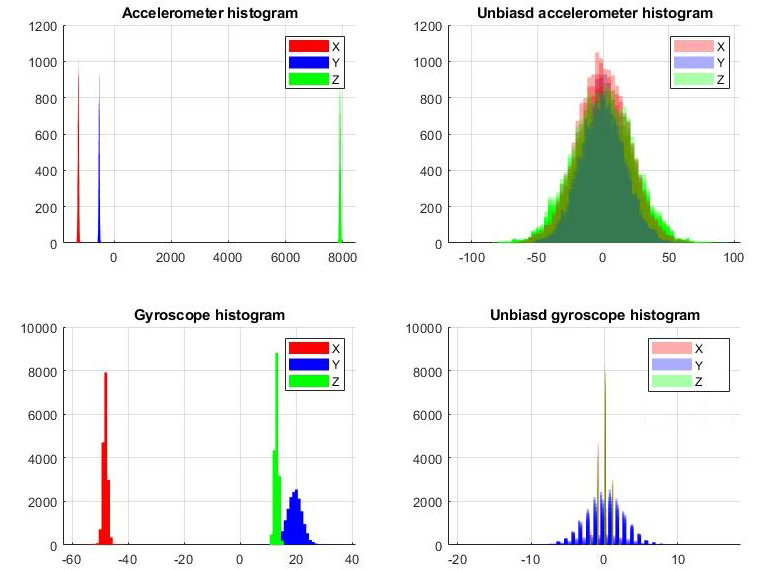
\includegraphics[width=0.7\linewidth]{kalman_histogram}
	\caption{هیستوگرام داده‌های حسگر حرکتی در حال سکون}
	\label{fig:kalman-histogram}
\end{figure}

ماتریس $Q$ اما در اکثر موارد مقداری قابل اندازه‌گیری نیست. شتاب نامعین حرکات دست به صورت اغتشاش ورودی مدل شده است که فرآیندی کاملاً نامعین است. اما با توجه به تأثیر مقدار $Q$ بر عملکرد فیلتر، می‌توان مقدار مناسبی را پیدا کرد. می‌دانیم هر چه کوواریانس اغتشاش ورودی را بزرگتر فرض کنیم، بدین معنی است که فیلتر باید بیشتر بر مشاهدات متکی باشد تا به پیش‌بینی. همچنین به عکس، اگر مقدار $Q$ کم باشد، فیلتر وزن بیشتری به پیش‌بینی خود از سیستم می‌دهد و اثر مشاهدات کمرنگ می‌شود. هرچه $Q$ کمتر باشد، عملکرد فیلتر لَخت‌تر و کندتر خواهد بود. هرچه $Q$ بزرگتر شود فیلتر حالت تهاجمی‌تری\footnote{\lr{Aggressive}} به خود می‌گیرد.

حال با در نظر گرفتن این مفهوم و عملکرد، برای تعیین $Q$ از روش سعی و خطا استفاده شد. بدین صورت که فیلتر کالمن با مقادیر مختلف $Q$ روی داده‌های از پیش ضبط شده شبیه‌سازی شد. سپس مقداری انتخاب شد که نه خیلی تهاجمی باشد و نه خیلی کند و حافظه‌دار. در نهایت برای حرکت خطی مقدار 8.0 $Q_{linear}=$ و برای حرکت دورانی مقدار 1.0 $Q_{rotational}=$ انتخاب شد.

شکل \ref{fig:kalman-accel-filtered-full} عملکرد فیلتر را روی داده‌های ضبط شده‌ی حرکت خطی نشان می‌دهد. همانطور که دیده می‌شود نویزهای موجود به خوبی حذف شده‌اند و داده‌ی خروجی فیلتر نویز مشهودی ندارد.

\begin{figure}[h]
	\centering
	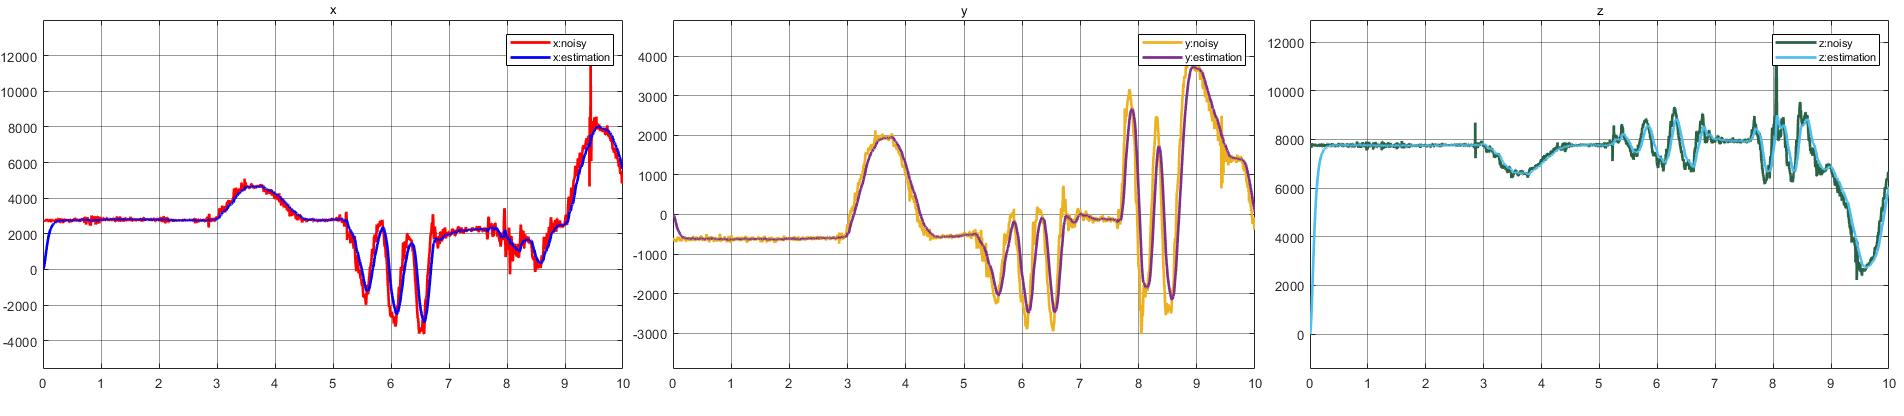
\includegraphics[width=\linewidth]{real_data_accel_full}
	\caption{خروجی خام شتاب خطی در مقایسه با مقدار فیلتر شده در هر سه محور}
	\label{fig:kalman-accel-filtered-full}
\end{figure}

حال که تمام مقادیر مورد نیاز فیلتر محاسبه شده و به دست آمدند، نوبت به پیاده‌سازی و بررسی عملکرد آن در ریزپردازنده می‌رسد. تمام معادلات مطابق آن چه در بالا گفته شد به صورت کد \lr{C} در ریزپردازنده پیاده شد. اما نکته‌ای وجود دارد.

می‌دانیم که معادلات سیستم دورانی (معادلات \ref{eq:rot-final}) نامتغیر با زمان هستند. لذا ماتریس‌های اصلی سیستم ($\phi$، $G$، $H$، $R$ و $Q$) نیز با زمان تغییر نمی‌کنند. حال به معادلات کالمن (\ref{eq:kalan-main}) توجه کنید. معادلات مربوط به بهره‌ی کالمن ($K$) و کوواریانس‌های خطا ($\Sigma(N+1|N+1)$ و $\Sigma(N+1|N)$) فقط تابع ماتریس‌های سیستم هستند و از حالت‌های سیستم مستقلند.

از طرفی می‌دانیم شرط کافی برای آنکه $\Sigma(N+1|N+1) = \Sigma(\infty)$ موجود باشد آن است که سیستم کنترل‌پذیر و رویت‌پذیر باشد و $Q$ و $R$ نیز مثبت باشند \cite{uncertain}. در اینجا شرط 0 $R,Q > $ برقرار است. در رابطه با سیستم حرکت دورانی داریم:

\begin{equation*}
	Ctrb(\phi, G) =
	\begin{bmatrix}
		0 & T \\
		1 & 1
	\end{bmatrix} \quad , \quad
	Obsv(\phi, H) =
	\begin{bmatrix}
		1 & 0 \\
		1 & T
	\end{bmatrix}
\end{equation*}

که هر دو مرتبه کامل هستند. در نتیجه هر دو سیستم کنترل‌پذیر و رویت‌پذیرند. بنابر این $\Sigma(\infty)$ موجود است که در نتیجه‌ی آن می‌توان گفت کوواریانس خطای پیش‌بینی و بهره‌ی کالمن نیز دارای حالت دائم و مقدار نهایی هستند.

دانستن اینکه بهره‌ی کالمن مقدار نهایی دارد و محاسبه‌ی آن مقدار، کمک می‌کند تا حالت گذرای فیلتر از بین برود و فیلتر از همان لحظه‌ی اول در بهینه‌ترین حالت کار کند. البته بزرگترین حسن آن است که دیگر نیازی به محاسبه‌ی $K$، $\Sigma(N+1|N)$ و $\Sigma(N+1|N+1)$ نیست. این امر حجم محاسبات را به شدت کاهش می‌دهد و سرعت پردازش را زیاد می‌کند. از این رو مقدار نهایی بهره‌ی کالمن توسط نرم‌افزار متلب محاسبه شد و مستقیما در معادله‌ی تخمین قرار داده شد. این کار حجم برنامه را 14 کیلوبایت کاهش داد (مجدد متذکر می‌شوم که حجم کل حافظه 64 کیلوبایت است!).


در نهایت با پیاده‌سازی فیلتر کالمن با روش جایگذاری مقداری نهایی بهره، اندازه‌گیری شتاب خطی و سرعت زاویه‌ای و فیلتر کردن آن بر روی ریزپردازنده به پایان می‌رسد. شکل \ref{fig:kalan-result-accel} نتیجه‌ی اجرای زمان-واقعی فیلتر برای شتاب خطی و شکل \ref{fig:kalan-result-gyro} نتیجه را برای سرعت زاویه‌ای نشان می‌دهند.

\begin{figure}[h]
	\centering
	\begin{subfigure}{0.8\textwidth}
		\centering
		\includegraphics[width=\linewidth]{accel_RT}
		\caption{شتاب خطی در سه محور}
		\label{fig:kalan-result-accel}
	\end{subfigure} \\
	\begin{subfigure}{\textwidth}
		\centering
		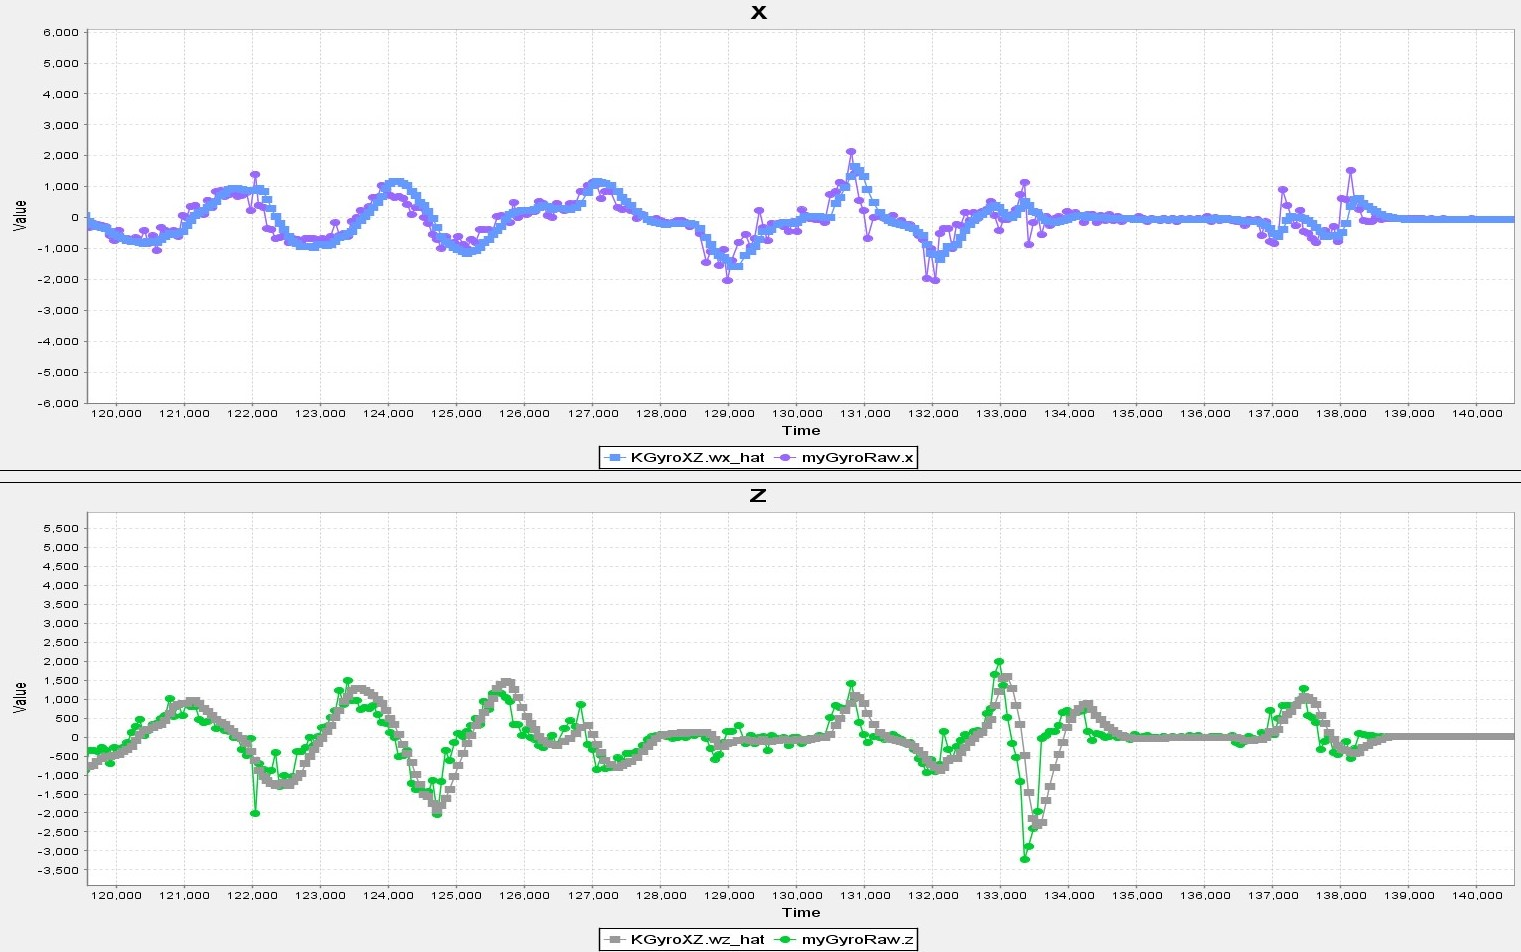
\includegraphics[width=0.8\linewidth]{gyro_RT}
		\caption{سرعت زاویه‌ای حول محورهای \lr{x} و \lr{z}}
		\label{fig:kalan-result-gyro}
	\end{subfigure}
	\caption{اجرای فیلتر کالمن روی ریزپردازنده و نتایج زمان-واقعی آن}
\end{figure}

\subsection{تشخیص گام}
برای تشخیص گام، ابتدا باید تخصیص محورهای مختصات حسگر را بررسی کنیم. طبق اطلاعات حسگر و با توجه به موقعیت نصب آن روی \pcbf، محورهای مختصات مطابق شکل \ref{fig:axis} روی ساعت قرار دارند.

\begin{figure}[h]
	\centering
	\includegraphics[width=0.5\linewidth]{axis}
	\caption{محورهای مختصات روی ساعت}
	\label{fig:axis}
\end{figure}

برای تشخیص گام، به شتاب خطی نیاز داریم. حسگر مورد استفاده در این پروژه این توانایی را دارد تا شتاب گرانش زمین را نیز در شتاب اندازه‌گیری شده گزارش کند. در واقع اگر حسگر را در حالت سکون قرار دهیم، اندازه‌ی جمع برداری شتاب در سه محور با $g$ برابر خواهد بود. از این ویژگی برای تخمین زاویه‌ی دست بهره بردم. به شکل \ref{fig:walk} توجه کنید.

\begin{figure}[h]
	\centering
	\begin{subfigure}{0.32\textwidth}
		\centering
		\includegraphics[width=\linewidth]{walk_3}
		\caption{}
		\label{fig:walk-3}
	\end{subfigure}
	\begin{subfigure}{0.3\textwidth}
		\centering
		\includegraphics[width=0.87\linewidth]{walk_2}
		\caption{}
		\label{fig:walk-2}
	\end{subfigure}
	\begin{subfigure}{0.3\textwidth}
		\centering
		\includegraphics[width=\linewidth]{walk_1}
		\caption{}
		\label{fig:walk-1}
	\end{subfigure}
	\caption{حالت‌های مختلف دست هنگام راه رفتن. به مؤلفه‌ی \lr{x} شتاب گرانش توجه کنید}
	\label{fig:walk}
\end{figure}
\newpage
هنگامی که دست در حالت \subref{fig:walk-2} قرار دارد، شتاب گرانش در راستای محور $y$ قرار دارد. در حالت \subref{fig:walk-3} اما به دلیل زاویه‌دار بودن دست، شتاب گرانش در دو راستای $x$ و $y$ تجزیه می‌شود. در این حالت مؤلفه‌ی $x$ مقداری مثبت دارد. به طور مشابه در حالت \subref{fig:walk-1} نیز شتاب گرانش در دو راستا تجزیه می‌شود و این بار مؤلفه‌ی $x$ مفداری منفی دارد. در نتیجه در هنگام راه رفتن خروجی حسگر حرکتی در راستای $x$ یک سیگنال شبه سینوسی خواهد بود که با عقب و جلو رفتن دست، کم و زیاد می‌شود. شکل \ref{fig:walk-x} خروجی یک نمونه سیگنال واقعی را نشان می‌دهد که توسط ساعت نمونه‌برداری شده و با متلب رسم شده است.

\begin{figure}[h]
	\centering
	\includegraphics[width=0.9\linewidth]{walk_x}
	\caption{شتاب خطی در راستای $x$ هنگام راه رفتن}
	\label{fig:walk-x}
\end{figure}

برای تشخیص گام از روی سیگنال فوق، از ایده‌ی منحنی پسماند\footnote{\lr{Hysteresis}} بهره بردم. در یک تعریف کلی، هیستِرِزیس عبارت است از وابستگی حالت یک سیستم به گذشته‌اش. سیستم‌های دارای هیسترزیس غیرخطی هستند، و مدلسازی ریاضی آنها می‌تواند بسیار سخت باشد \cite{hister}.

در این قسمت یک حد بالا و یک حد پایین تعریف می‌شود. هرگاه شتاب در راستای $x$ از حد بالا گذر کند و بیشتر شود، یک متغیر یا \lr{flag} یک می‌شود. این متغیر حالت قبلی خود را حفظ می‌کند تا آنجا که شتاب از حد پایینی گذر کند و کمتر شود. در این صورت مقدار صفر به خود می‌گیرد تا صبر می‌کند تا مجدد از حد بالا بگذرد.

به شکل \ref{fig:walk-hister} توجه کنید. در نمودار بالا، سیگنال حسگر با رنگ قرمز، حد بالا با رنگ آبی و حد پایین با رنگ بنفش مشخص شده‌اند. نمودار پایین مربوطه به پرچم مورد نظر است. همانطور که گفته شد، پرچم فقط وقتی تغییر وضعیت می‌دهد که شتاب یا از حد بالا فراتر رود یا از حد پایین کمتر شود. در صورتی که شتاب در محدوده‌ی بین این دو باشد، پرچم وضعیت قبلی را حفظ می‌کند.

اکنون کافی است تا به سیگنال پرچم دقت کنیم. هر لبه‌ی بالارونده در آن  به معنای برداشتن یک گام توسط کاربر است. پس باید هنگامی که پرچم یک می‌شود، یک عدد به متغیر تعداد گام اضافه کرد.

\newpage
\begin{figure}[h]
	\centering
	\includegraphics[width=0.87\linewidth]{walk_hister}
	\caption{سیگنال شتاب خطی راستای $x$ در کنار حدود پسماند و متغیر پرچم}
	\label{fig:walk-hister}
\end{figure}

\subsection{تشخیص چرخش دست}
فرآیند تشخیص چرخش دست برای روشن صفحه نمایش بسیار مشابه فرآیند تشخیص گام است. با این تفاوت که هنگام چرخش دست و بالا آمدن آن، با توجه به محورهای حسگر (شکل \ref{fig:axis}) یک چرخش اساسی حول محور $y$ رخ می‌دهد. بدیهی است که سایر محورها نیز سرعت و شتاب دارند، اما اندازه‌گیری سرعت زاویه‌ای حول محور $y$ به تنهایی کافی است. زیرا حرکت روزمره‌ای که بتواند چرخش حول ساعد دست را ایجاد کند تا ساعت به اشتباه بیفتد بسیار نادر است. اکثر چرخش‌های دست حول دیگر محورها صورت می‌گیرند.

\begin{figure}[h]
	\centering
	\includegraphics[width=0.87\linewidth]{screen_hister}
	\caption{سیگنال سرعت زاویه‌ای حول محور $y$ در کنار حدود پسماند و متغیر پرچم}
	\label{fig:screen-hister}
\end{figure}

به شکل \ref{fig:screen-hister} توجه کنید. مشابه حالت تشخیص گام، در نمودار بالا سیگنال حسگر با رنگ قرمز، حد بالا با رنگ آبی و حد پایین با رنگ بنفش مشخص شده‌اند. نمودار پایین مربوطه به پرچم مورد نظر است. همانطور که گفته شد، پرچم فقط وقتی تغییر وضعیت می‌دهد که سرعت زاویه‌ای یا از حد بالا فراتر رود یا از حد پایین کمتر شود. در صورتی که سرعت زاویه‌ای در محدوده‌ی بین این دو باشد، پرچم وضعیت قبلی را حفظ می‌کند.

اکنون کافی است تا به سیگنال پرچم دقت کنیم. هر لبه‌ی بالارونده در آن  به معنای چرخش دست حول ساعد یا همان محور $y$ توسط کاربر است. پس باید هنگامی که پرچم یک می‌شود، فرمان روشن شدن صفحه نمایش نیز صادر شود.

\section{ارتباطات} \label{sec:comm}
در این بخش به بررسی نحوه‌ی ارتباط ساعت با گوشی و پروتکل‌های ارتباطی می‌پردازیم. می‌دانیم که بستر ارتباطی ساعت با گوشی، بلوتوث است. سرعت ارتباط روی 115200 بیت بر ثانیه تنظیم شده است. اکنون باید زبان مشترکی بین ساعت و گوشی تعریف کرد تا تحت آن به تبادل داده بپردازند. ابتدا وظایفی که هرکدام از طرفین ارتباط برعهده دارند را بررسی می‌کنیم.
\begin{itemize}
	\item ساعت
	\begin{enumerate}
		\item ارسال میزان شارژ باتری
		\item ارسال تعداد قدم‌های طی شده
		\item ارسال تایید ارتباط به گوشی
		\item ارسال داده‌های حسگر \lr{PPG}
	\end{enumerate}
	\item گوشی
	\begin{enumerate}
		\item ارسال درخواست ارتباط
		\item ارسال نام کاربری
		\item ارسال ساعت و تاریخ
		\item ارسال تنظیمات آلارم
		\item ارسال نتایج الگوریتم‌های پردازش \lr{PPG} شامل ضربان قلب و سطح اکسیژن خون
		\item ارسال مداوم سیگنال اتصال
	\end{enumerate}	
\end{itemize}

\newpage
برای انجام وظایف فوق، پروتکل ارتباطی‌ای میان ساعت و گوشی تعریف شد. این پروتکل شامل تعریف چند بسته داده‌ی معتبر است که هر دو سمت ارتباط موظف به رعایت آن هستند. در ادامه این بسته‌ها شرح داده می‌شوند.

\subsection{بسته‌ی درخواست ارتباط}
تست

\subsection{بسته‌ی تنظیم نام کاربری}
تست

\subsection{بسته‌ی تنظیم ساعت و تاریخ}
تست

\subsection{بسته‌ی تنظیم آلارم}
تست

\subsection{بسته‌ی نتایج پردازش}
تست

\subsection{بسته‌ی بررسی ارتباط}
تست

\subsection{بسته‌ی داده‌های حسگر \lr{PPG} و تنظیمات ساعت}
تست






